\documentclass
[
	paper=A4,					% paper size --> A4 is default in Germany
	twoside=true,				% onesite or twoside printing
	openright,					% doublepage cleaning ends up right side
	parskip=full,				% spacing value / method for paragraphs
	chapterprefix=true,			% prefix for chapter marks
	12pt,						% font size
	headings=normal,			% size of headings
	bibliography=totoc,			% include bib in toc
	listof=totoc,				% include listof entries in toc
	titlepage=on,				% own page for each title page
	captions=tableabove,		% display table captions above the float env
	draft=false,				% value for draft version
]
{scrreprt}

%Text encryption
\usepackage[T2A, T1]{fontenc}
\usepackage[utf8]{inputenc}

\newcommand{\thesisTitle}{Управление на български робот РОБКО 01 с ARM-базиран микроконтролер STM32L476RG и отдалечен достъп през интернет}
\newcommand{\thesisAuthor}{Владимир Гаристов}
\newcommand{\thesisSupervisor}{маг. инж. Росен Витанов}
\newcommand{\thesisReviewer}{}
\newcommand{\thesisSubject}{\thesisTitle}
\newcommand{\thesisDate}{8 Декември 2017}
\newcommand{\thesisVersion}{0.4}
\newcommand{\thesisUniversity}{Технически Университет - София}
\newcommand{\thesisSchool}{Технологично Училище "Електронни Системи"}
\newcommand{\thesisFaculty}{Факултет "Електронна Техника и Технологии"}
\newcommand{\thesisDepartment}{Катедра "Електронна Техника"}

%Subject застава над заглавието
\subject{\Large\thesisSchool\\ към \thesisUniversity\newline\newline}
\title{\thesisTitle}
\author{\thesisAuthor}
\date{}

\makeatletter
\newcommand*{\textoverline}[1]{$\overline{\hbox{#1}}\m@th$}
\makeatother

\PassOptionsToPackage{dvipsnames}{xcolor}

%Used packages
\usepackage{minted}
\usepackage{color}
\usepackage{graphicx}
\usepackage{caption}
\usepackage{subcaption}
\usepackage[main=bulgarian,english]{babel}
\usepackage{pdfpages}
\usepackage{placeins}
\usepackage{multirow}
\usepackage{makecell}
\usepackage{array}
\usepackage{amsmath}
\usepackage{textcomp}
\usepackage{tikz}
\usepackage
[                           % clean thesis style
	figuresep=colon,
	sansserif=false,
	hangfigurecaption=false,
	hangsection=true,
	hangsubsection=true,
	colorize=full,
	colortheme=bluegreen,
	bibsys=biber,
	bibfile=references.bib,
	bibstyle=numeric
]
{cleanthesis}

\hypersetup
{					            % setup the hyperref-package options
	pdftitle={\thesisTitle},	% 	- title (PDF meta)
	pdfsubject={\thesisSubject},% 	- subject (PDF meta)
	pdfauthor={\thesisAuthor},	% 	- author (PDF meta)
	plainpages=false,			% 	-
	colorlinks=false,			% 	- colorize links?
	pdfborder={0 0 0},			% 	-
	breaklinks=true,			% 	- allow line break inside links
	bookmarksnumbered=true,		%
	bookmarksopen=true,			%
	unicode=true                % non-Latin characters in Acrobat’s bookmarks
}

\newcolumntype{L}[1]{>{\raggedright\let\newline\\\arraybackslash\hspace{0pt}}m{#1}}
\newcolumntype{C}[1]{>{\centering\let\newline\\\arraybackslash\hspace{0pt}}m{#1}}
\newcolumntype{R}[1]{>{\raggedleft\let\newline\\\arraybackslash\hspace{0pt}}m{#1}}

\usetikzlibrary{shapes.geometric, arrows}
\tikzstyle{startstop} = [rectangle, rounded corners, minimum width=3cm, minimum height=1cm,text centered, draw=black, fill=red!30]
\tikzstyle{io} = [trapezium, trapezium left angle=70, trapezium right angle=110, minimum width=3cm, minimum height=1cm, text centered, draw=black, fill=blue!30]
\tikzstyle{process} = [rectangle, minimum width=3cm, minimum height=1cm, text centered, draw=black, fill=orange!30]
\tikzstyle{decision} = [diamond, minimum width=1cm, minimum height=1cm, text centered, draw=black, fill=green!30, inner sep = -0.4cm]
\tikzstyle{arrow} = [thick,->,>=stealth]
\tikzstyle{arrow_no_head} = [thick]

\begin{document}

\pagestyle{plain}

%\maketitle

\includepdf[pages={1}]{documents/title_page.pdf}
\cleardoublepage
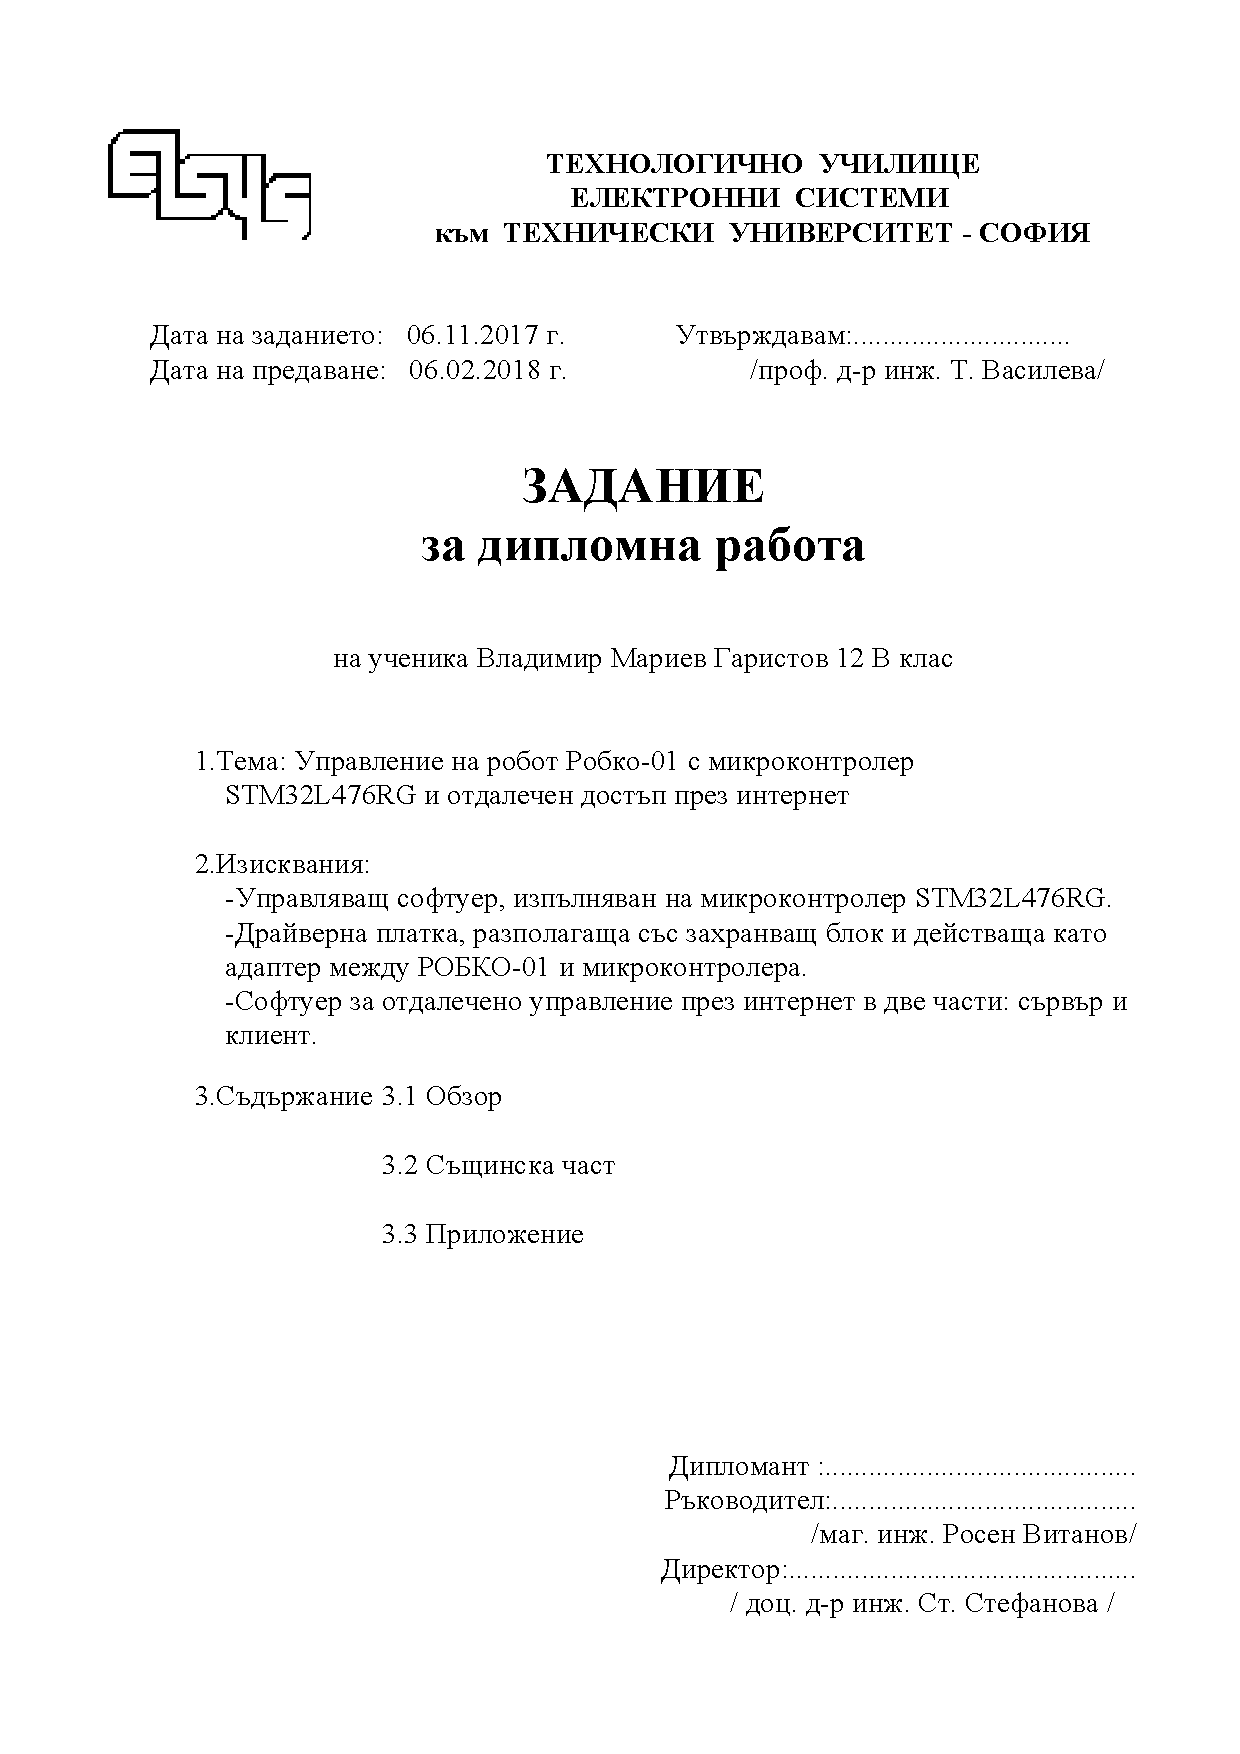
\includepdf[pages={1}]{documents/zadanie.pdf}
\cleardoublepage
\tableofcontents
\listoffigures
\listoftables

\begin{center}
    {\large \bigskip \bigskip Благодарности на\\маг. инж. Константин Несторов,\\маг. инж. Иван Учерджиев и\\гл. ас. др. инж. Димитър Николов}
\end{center}

\pagestyle{maincontentstyle}

\chapter{РОБКО 01}
\section{История}
През 80-те години на 20-ти век в България се наблюдава бурно развитие на електрониката.
\cite{NRB_electronics}
Управляваната от компютри автоматика навлиза все повече в индустрията. Поради нуждата от квалифицирани специалисти по автоматика и мехатроника е създадена серията учебни роботи РОБКО. Представляват неголеми механизми, задвижвани от стъпкови електродвигатели. Наподобяват индустриални роботи. Предназначени са да се управляват от персонален компютър Правец 82 или ИМКО-2.\\
\indent{} %те са еднакви
Серията РОБКО е разработена в Института по Техническа Кибернетика и Роботика към Българската Академия на Науките (ИТКР-БАН) и произвеждана от Завод за медицинса техника в град София. Повечето модели РОБКО са еквиваленти на проектирани в западна Европа и САЩ роботи. Например РОБКО 9 е копие на Heathkit HERO 1, а РОБКО 10 силно наподобява Microbot TeachMover.
\cite{robko-obscomp-history}
Първият робот от серията - РОБКО 01 (показан на фиг. \ref{fig:robko01_mini_mover}) е директно копие на американския робот Mini-mover 5. Той е най-популярният РОБКО, произведени са между 4 и 17 хиляди броя.
\cite{robko-obscomp-history}\\
\indent{}
\begin{figure}
    \centering
    \begin{subfigure}{1\textwidth}
        \centering
        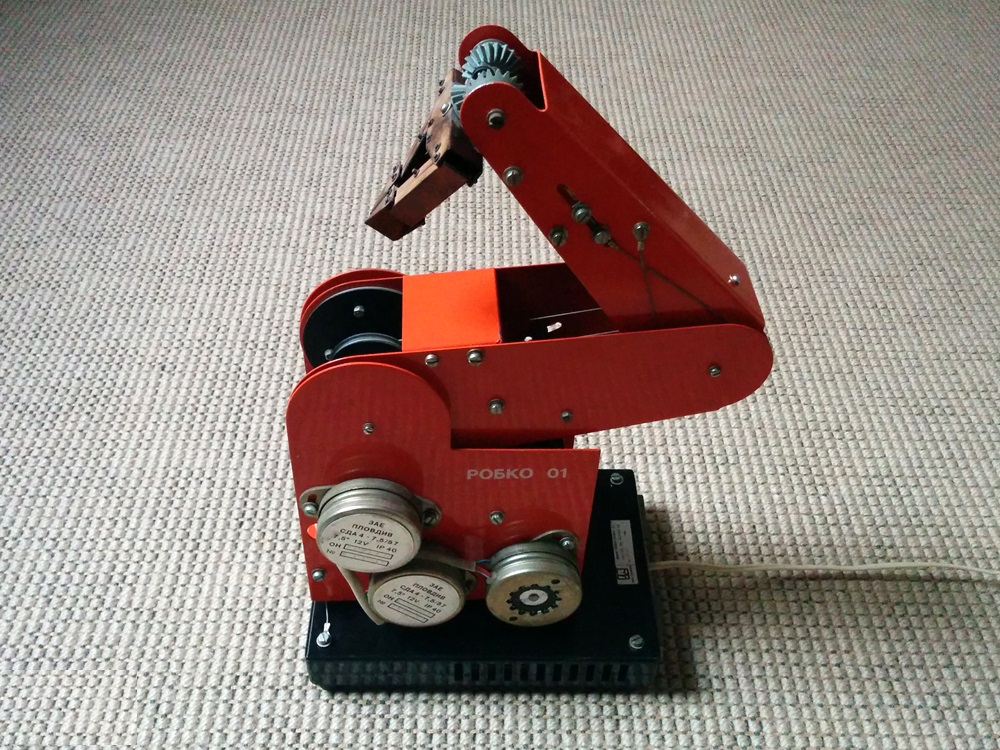
\includegraphics[width=.7\linewidth]{pictures/robko01.jpg}
        \caption{РОБКО 01}
        \label{fig:robko01}
    \end{subfigure}
    \par\bigskip
    \begin{subfigure}{1\textwidth}
        \centering
        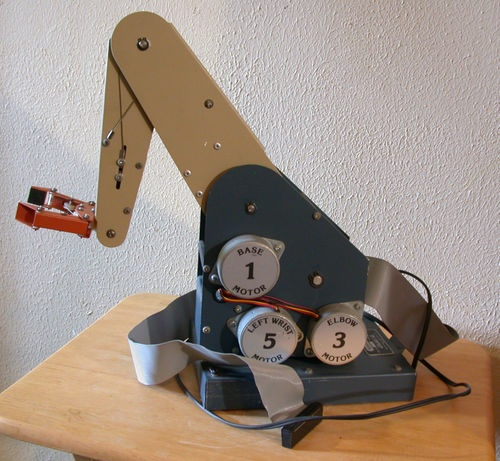
\includegraphics[width=.7\linewidth]{pictures/mini_mover.jpg}
        \caption{Mini-mover 5}
        \label{fig:mini_mover}
    \end{subfigure}
    \caption{РОБКО 01 и Mini-mover 5}
    \label{fig:robko01_mini_mover}
\end{figure}
Серията РОБКО включва въртяща се маса и конвейер (фиг. \ref{fig:turntable}), вариант на РОБКО 01 с монтирани на ставите мотори вместо метални жила за предаване на движението (фиг. \ref{fig:robko_alt}), модел със собствена работна маса (фиг. \ref{fig:robko_vela}), робот с деликатна щипка за стъкленици (фиг. \ref{fig:robko_lab}) и подобен на кран робот (фиг. \ref{fig:collection}, горе-ляво и център-дясно).
\begin{figure}
    \centering
    \begin{subfigure}{0.45\textwidth}
        \centering
        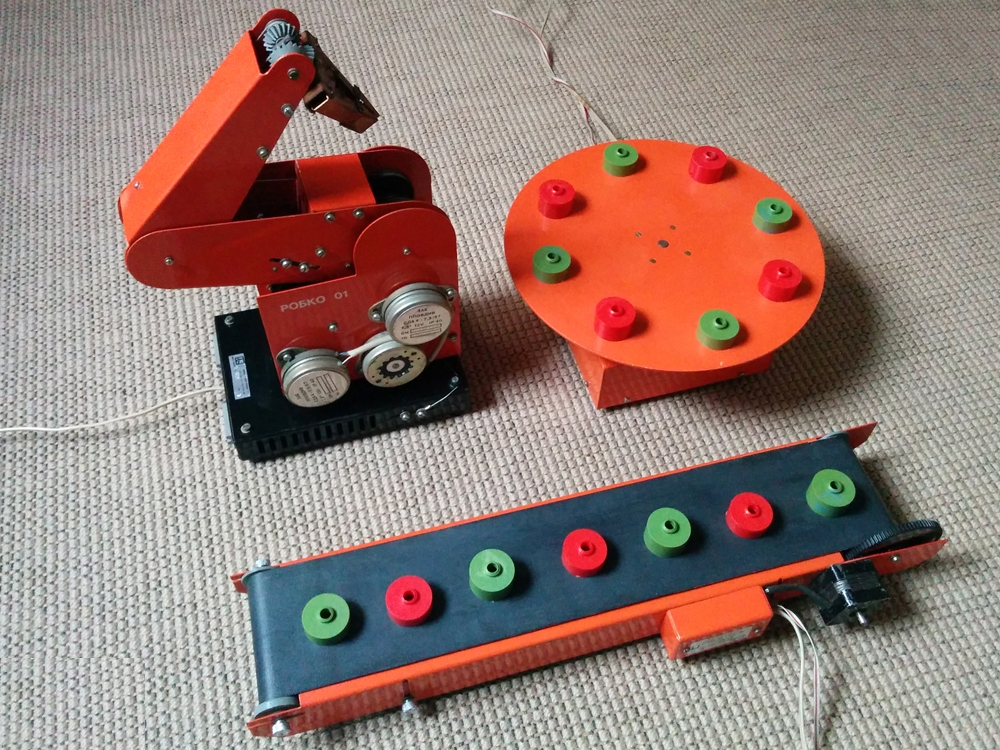
\includegraphics[width=\linewidth]{pictures/turntable_conveyor.jpg}
        \caption{Въртяща се маса и конвейер}
        \label{fig:turntable}
    \end{subfigure}
    \hfill%
    \begin{subfigure}{0.45\textwidth}
        \centering
        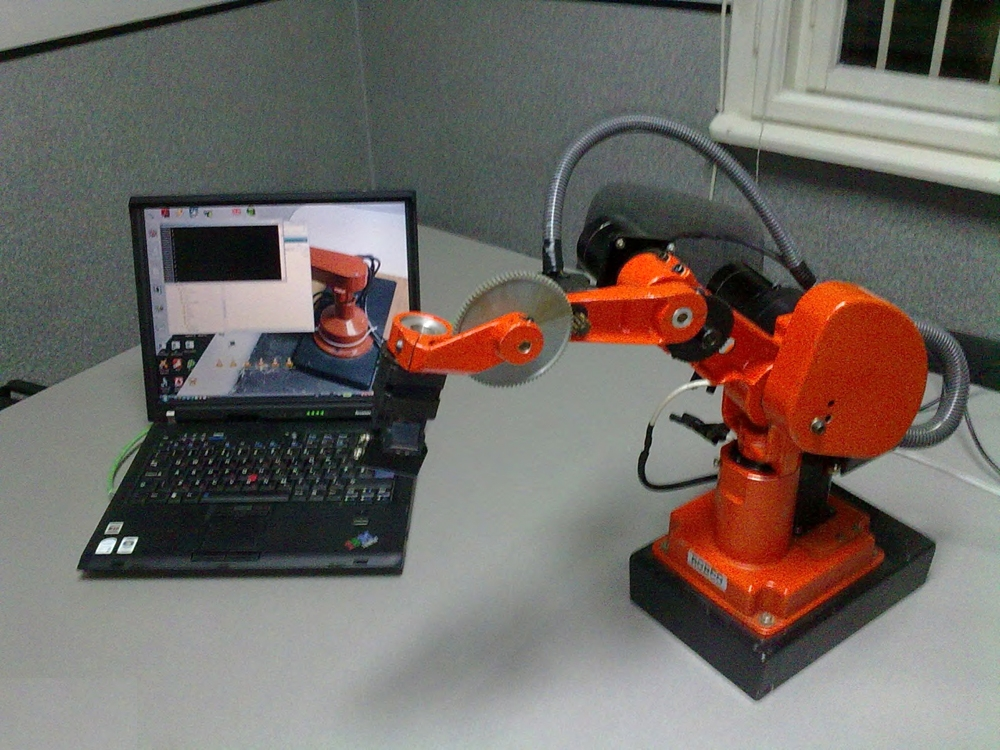
\includegraphics[width=\linewidth]{pictures/robko_alt.jpg}
        \caption{Подобен на РОБКО 01 модел}
        \label{fig:robko_alt}
    \end{subfigure}
    \par\bigskip
    \begin{subfigure}{0.45\textwidth}
        \centering
        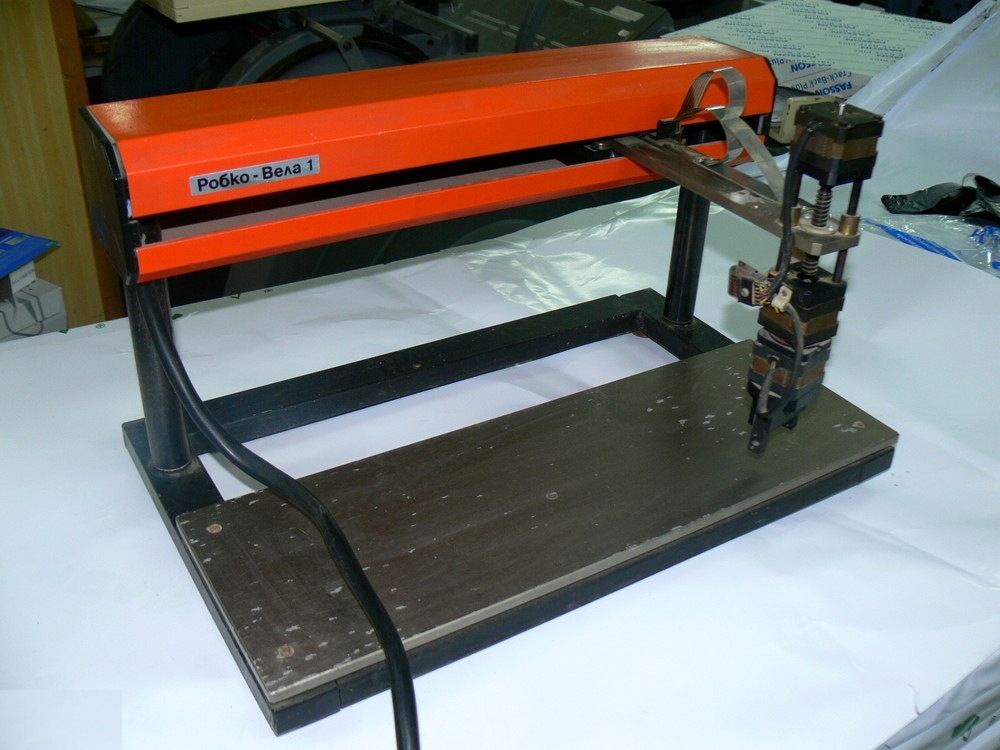
\includegraphics[width=\linewidth]{pictures/robko_vela.jpg}
        \caption{РОБКО Вела 1}
        \label{fig:robko_vela}
    \end{subfigure}
    \hfill%
    \begin{subfigure}{0.45\textwidth}
        \centering
        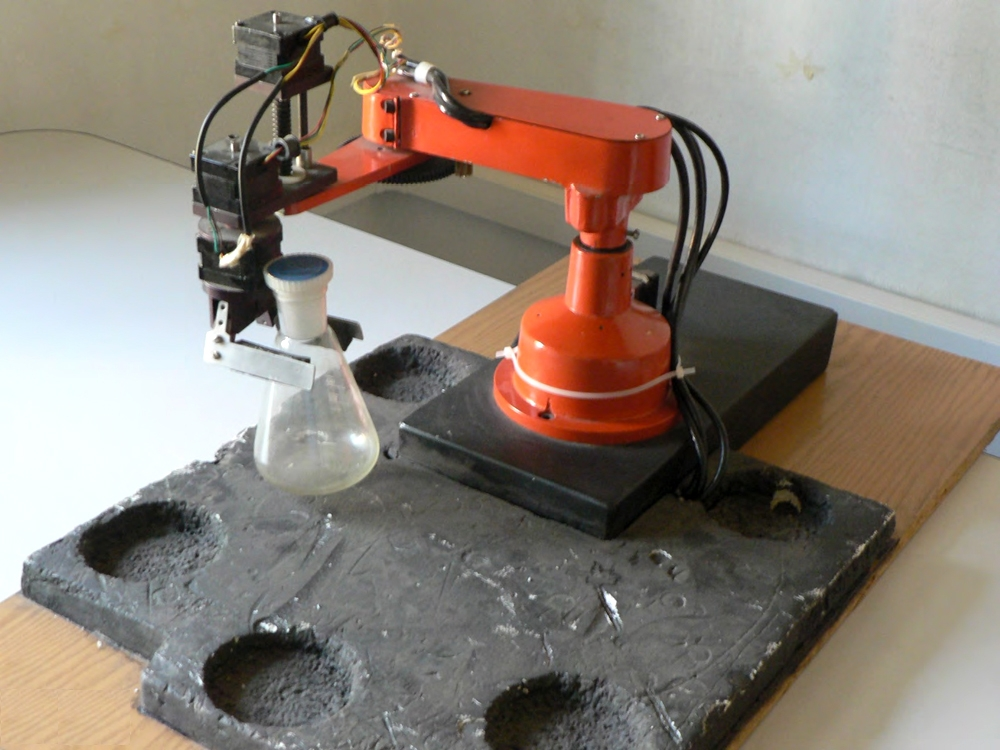
\includegraphics[width=\linewidth]{pictures/robko_lab.jpg}
        \caption{Лабораторен модел}
        \label{fig:robko_lab}
    \end{subfigure}
    \caption{Различни модели от серията РОБКО}
    \label{fig:robko_series}
\end{figure}
\begin{figure}
    \centering
    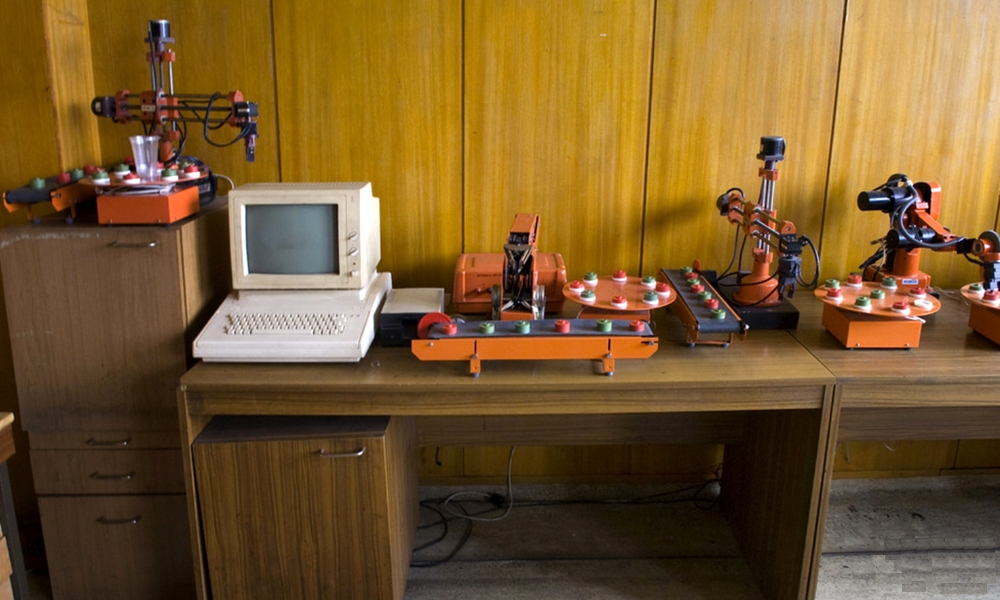
\includegraphics[width=\linewidth]{pictures/robko_collection.jpg}
    \caption{Колекция от различни модели РОБКО и Правец 8М}
    \label{fig:collection}
\end{figure}
Произвеждани са захранващ блок (фиг. \ref{fig:robko_psu}) и три различни накрайника за РОБКО 01 - обикновен хващач, оптичен сензорен хващач (фиг. \ref{fig:robko_opto}) и електромагнит (фиг. \ref{fig:robko_em}). Оптичният сензорен хващач се разглежда подробно в точка \ref{opto_claw_section}.
\begin{figure}
    \centering
    \begin{subfigure}{0.7\textwidth}
        \centering
        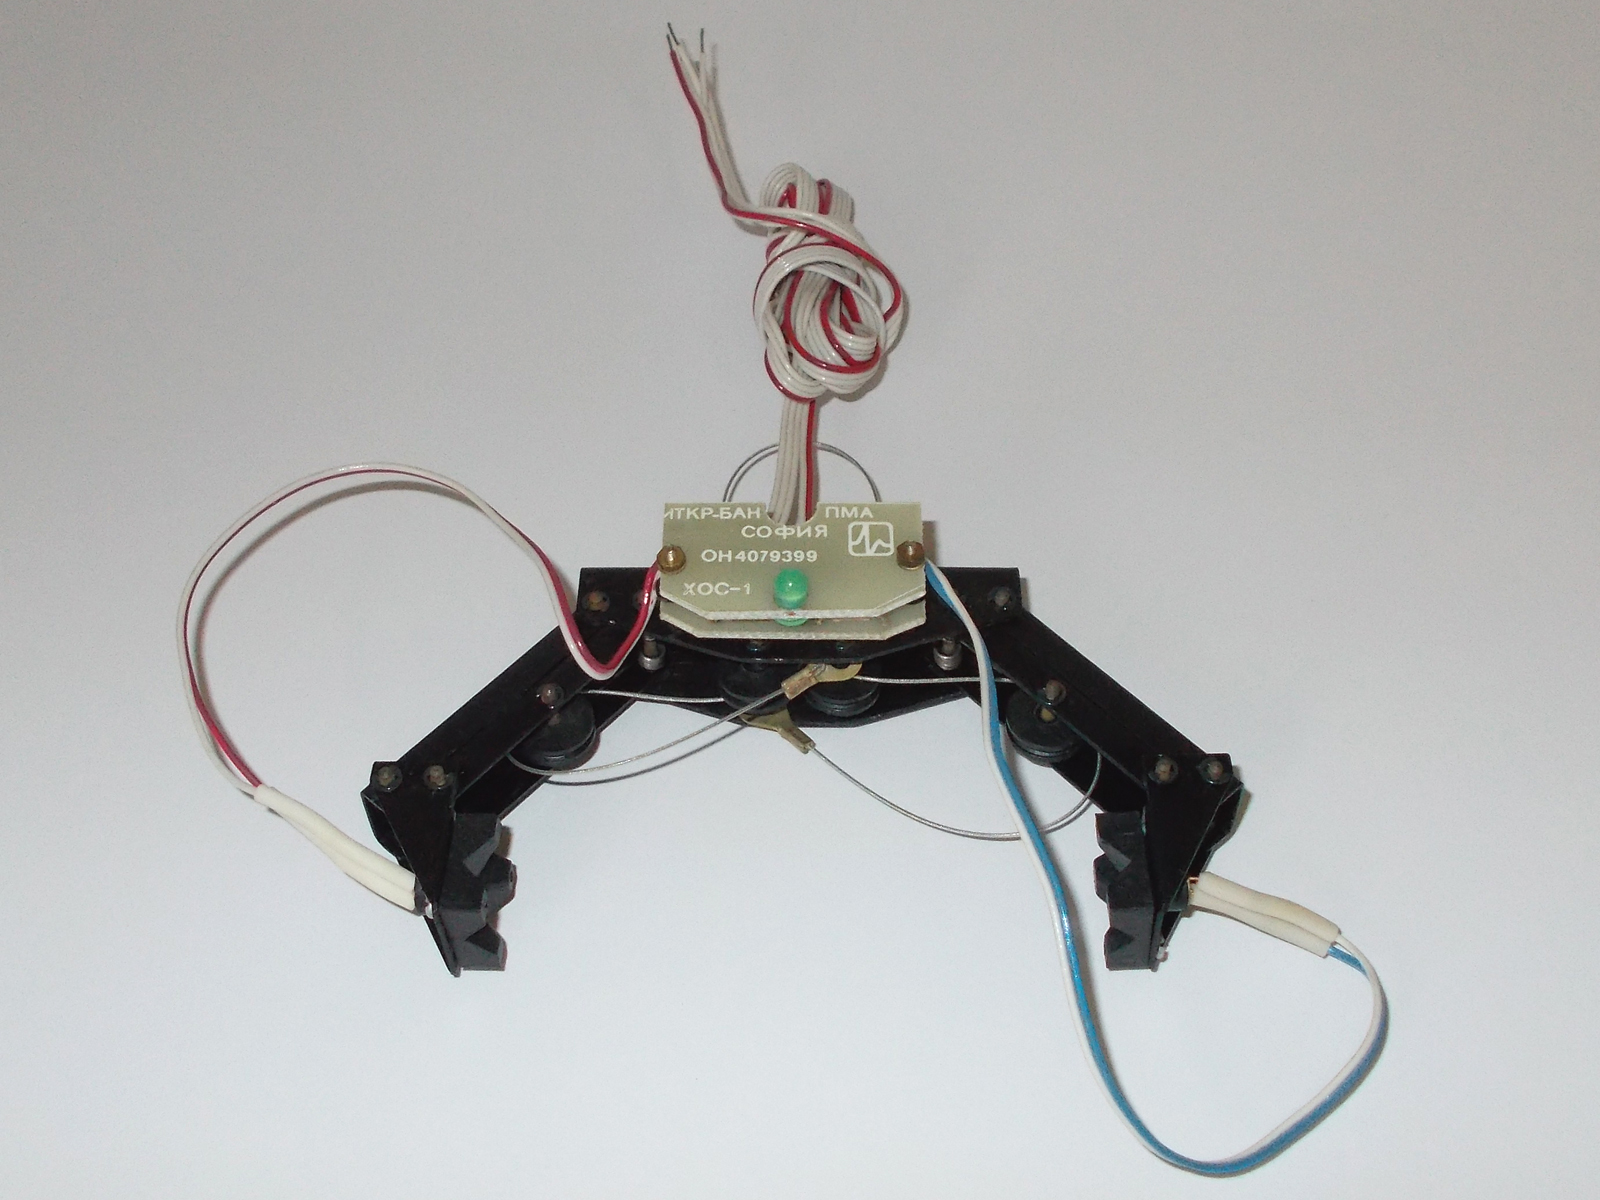
\includegraphics[width=\linewidth]{pictures/robko_opto_claw.jpg}
        \caption{Оптичен сензорен хващач}
        \label{fig:robko_opto}
    \end{subfigure}
    \par\bigskip
    \begin{subfigure}{0.45\textwidth}
        \centering
        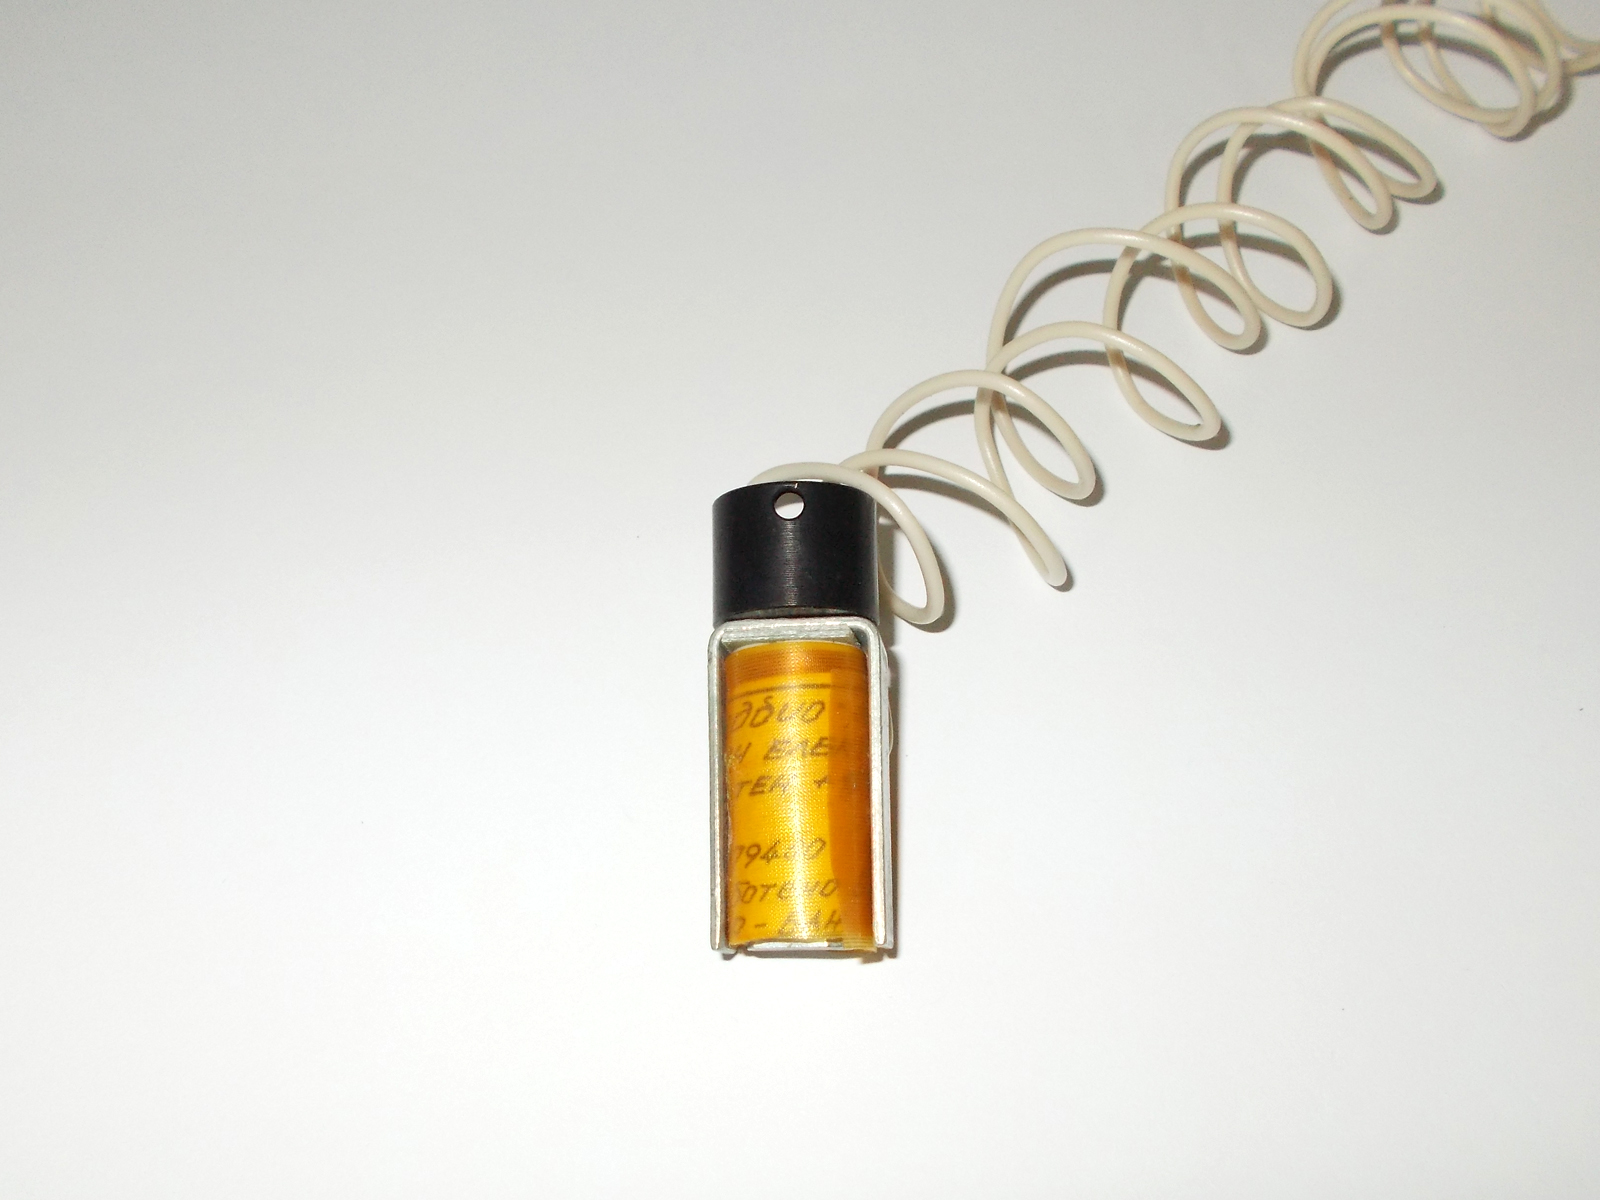
\includegraphics[width=\linewidth]{pictures/robko_electromagnet.jpg}
        \caption{Електромагнит}
        \label{fig:robko_em}
    \end{subfigure}
    \hfill%
    \begin{subfigure}{0.45\textwidth}
        \centering
        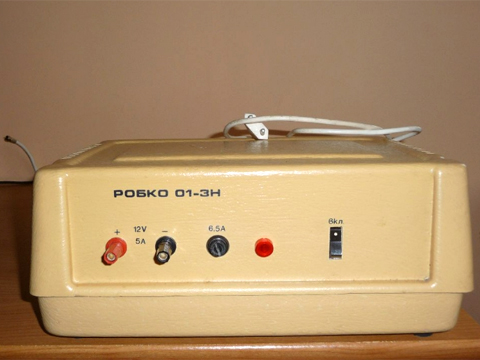
\includegraphics[width=\linewidth]{pictures/robko_psu.jpg}
        \caption{Захранващ модул}
        \label{fig:robko_psu}
    \end{subfigure}
    \caption{Аксесоари за РОБКО 01}
    \label{fig:robko_accessories}
\end{figure}
\section{РОБКО 01 в настоящето}
Малкото запазени екземпляри от серията РОБКО почти винаги са от модел 01 или комплект въртяща се маса и конвейер. Съществуват различни проекти, успешно реализирали управление на РОБКО 01. Някои от тях се свързват с драйверната платка на робота, а други я заменят. Разработени са различни потребителски интерфейси: програми с графична среда, програми с команден ред и управление с джойс
тици.\\\indent{}
РОБКО 01 е проектиран да се управлява от ИМКО-2/Правец82 чрез разширителната карта показана на фигура \ref{fig:orig_cntrl}. Повечето модерни РОБКО проекти заменят тази платка с микроконтролер.\\
\begin{figure}
    \centering
    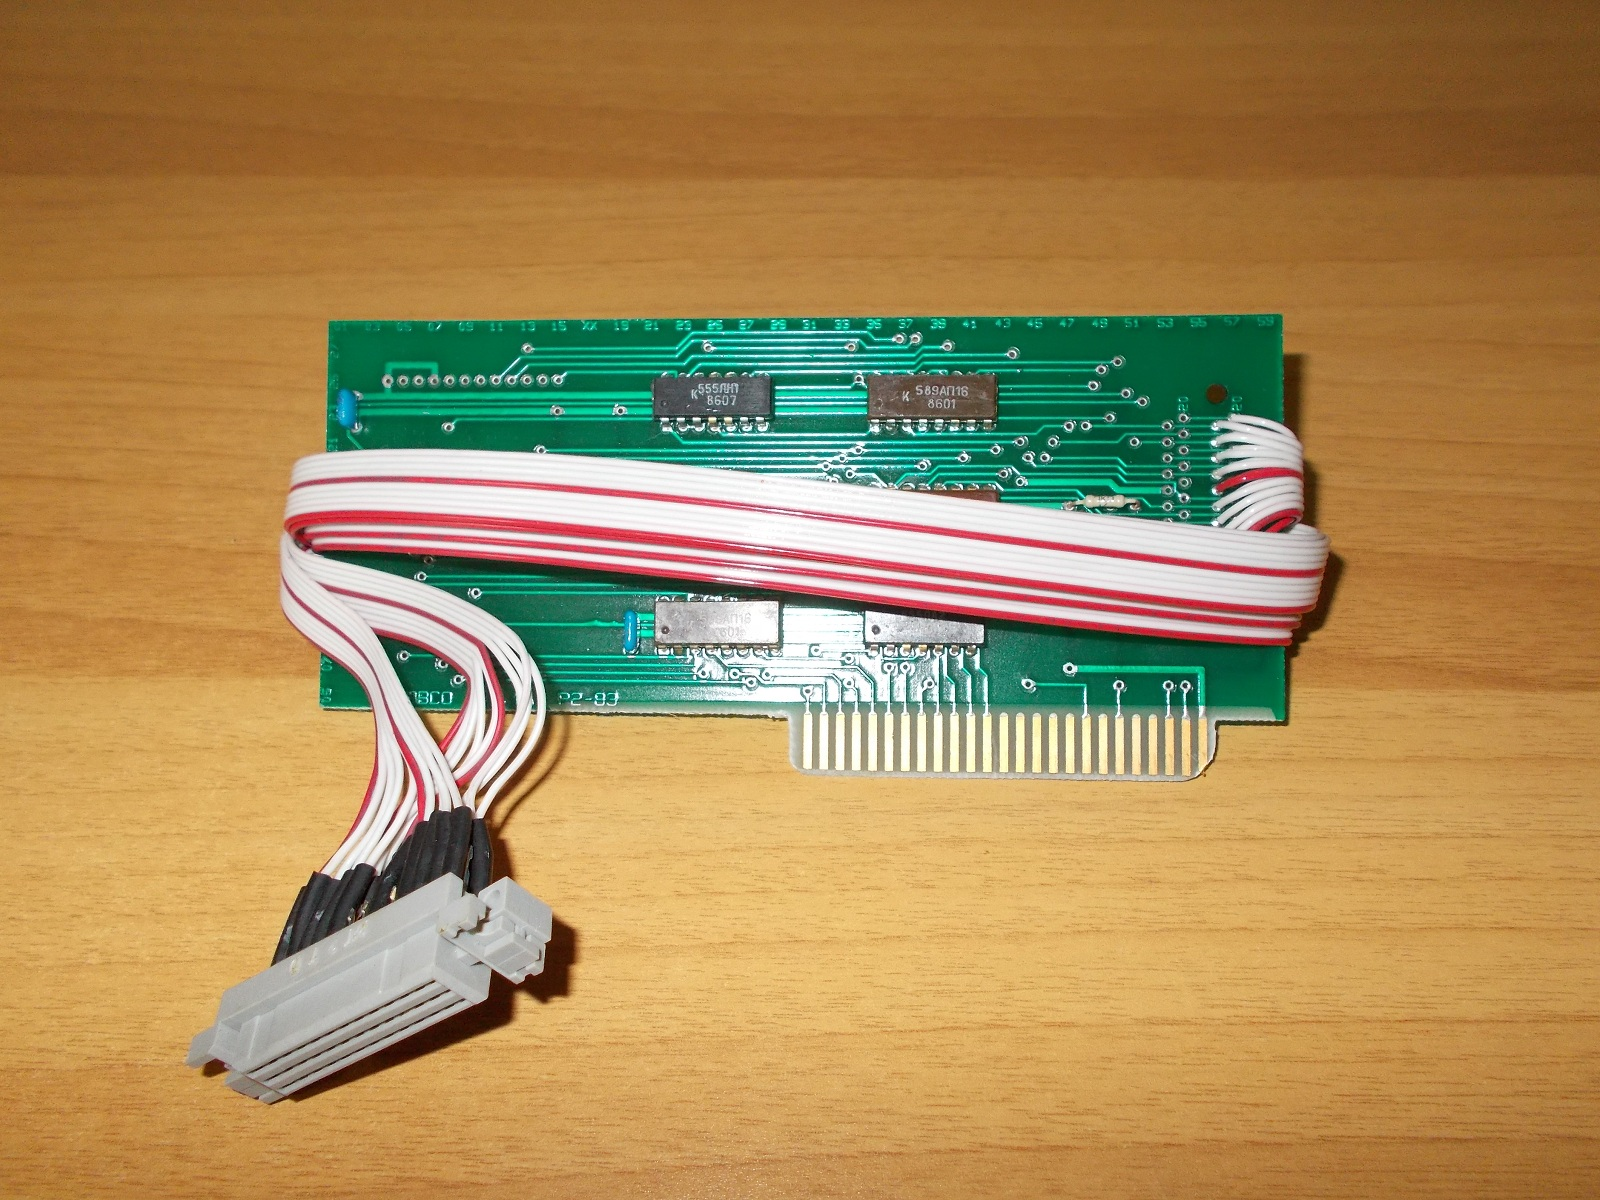
\includegraphics[width=\linewidth]{pictures/robko_orig_controller.jpg}
    \caption{Разширителна карта за ИМКО-2/Правец82, свързваща се с драйверната платка на РОБКО 01}
    \label{fig:orig_cntrl}
\end{figure}

Пример за такава реализация е проектът на Валентин Николов.
\cite{robko-val_niko}
Проектираната от него платка (фиг. \ref{fig:usb_cntrl}) е базирана на микроконтролер PIC4620 от Microchip. Разполага с бутони за ръчно управление и връзка с компютър през USB интерфейс. Неговият софтуер, изпълняван на персонален компютър, предоставя графична среда за управление на робота. Може да се контролира от мишка, клавиатура или джойстик и позволява едновременно движение на повече от един мотор. Демонстрация на функционалностите на проекта на Валентин Николов е налична в интернет.\cite{robko-usb-gui}
\begin{figure}
    \centering
    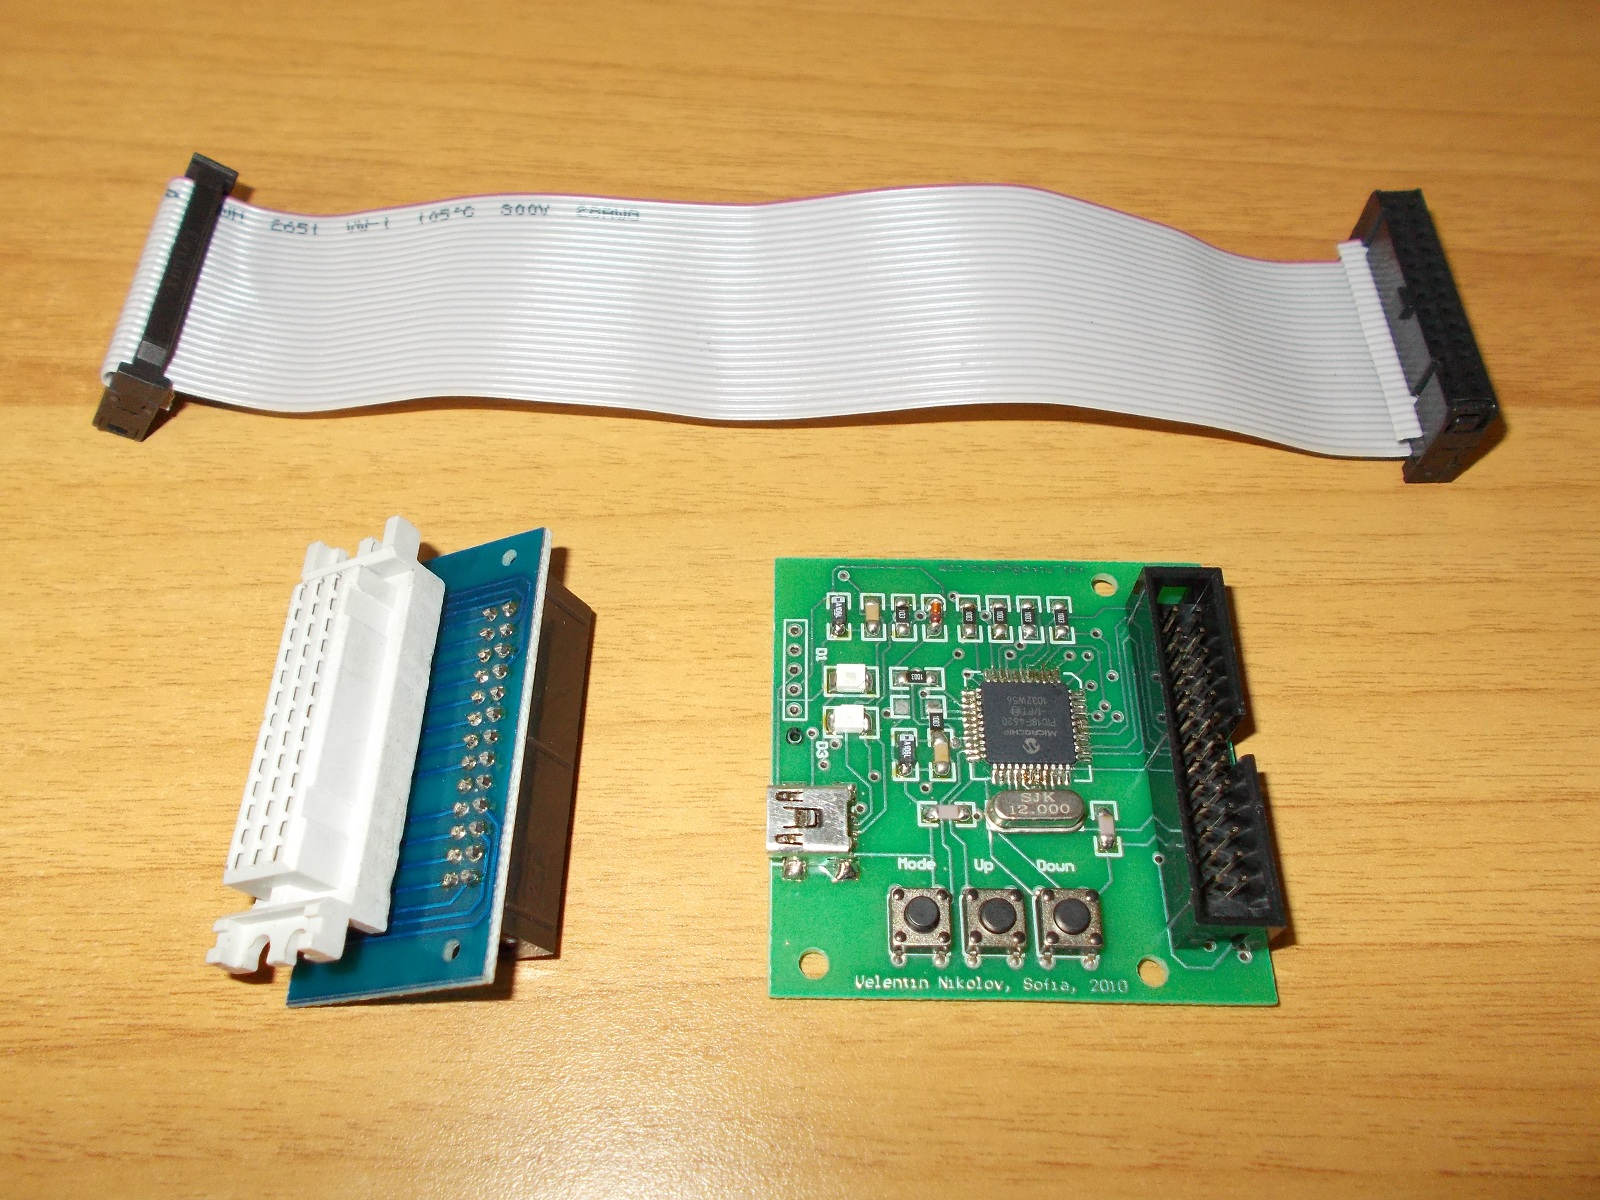
\includegraphics[width=\linewidth]{pictures/robko_usb_controller.jpg}
    \caption{Микроконтролерна платка, свързваща драйверната платка на РОБКО 01 с персонален компютър}
    \label{fig:usb_cntrl}
\end{figure}

Подобна система е разработена от Орлин Димитров - студент в Технически Университет - Габрово. Контролерът, използван от него, е Arduino UNO. Микроконтролерната платка се свързва към РОБКО 01 и към персонален компютър, подаващ команди през серийна връзка. Роботът се управлява от програма с графична среда, изпълнявана на персоналния компютър. Софтуерът позволява както ръчно управление, така и изпълнение на поредица от предварително зададени движения. Отличителна черта на тази система е способнастта й плавно да ускорява и забавя въртенето на моторите.
\cite{robko-orlin-fb}
Проектът на Орлин Димитров е единственият известен в интернет, успешно реализирал едновременното управление на повече от един РОБКО 01.
\cite{robko-orlin-double2}

Друг подход за управлението на РОБКО 01 е да се подмени драйверната платка на робота. Този метод е приложен от Симеон Иванов, студент от Русенският университет "Ангел Кънчев".
\cite{robko-atmega128}
Разработената от него платка (показана на фигура \ref{fig:new_cntrl_brd}) се монтира на мястото на оригиналната драйверна платка в основата на робота. Включва в себе си микроконтролер ATMega128, Ethernet контролер ENC424J600, захранващ блок, шест интегрални схеми за управление на стъпкови мотори и интегрални схеми за комуникация по UART, RS232 и USB. Тази разработка е най-функционалната имплементация на РОБКО 01 сред известните в интернет такива.\\
\indent{}
Контролерът комуникира с персонален компютър по ModBUS протокол, който е стандартен за автоматизацията в индустриални условия. Това позволява отдалечено управление на робота по интернет. Могат да се движат множество мотори едновременно. Софтуерът на микроконтролерът извършва изчисления за права и обратна кинематика - може да позиционира щипката на робота на зададени координати и да определя текущото местоположение. Командите към контролера се подават под формата на G код. Това на практика превръща РОБКО 01 в CNC (Цифрово-Програмно Управляема) машина. Тази способност на разработката е показана на видеоклип в интернет.
\cite{robko-cnc}
\begin{figure}
    \centering
    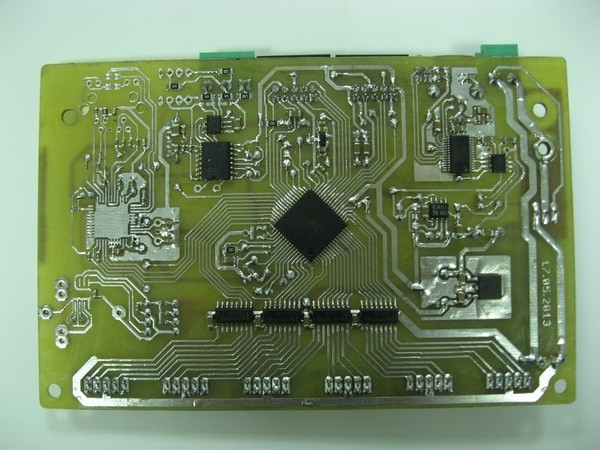
\includegraphics[width=\linewidth]{pictures/robko_new_driver_board.jpg}
    \caption{Платка, заменяща оригиналната драйверна платка на РОБКО 01}
    \label{fig:new_cntrl_brd}
\end{figure}
\section{Настояща разработка}
Целта на настоящия проект е да се проектира и изработи управляващо устройство за РОБКО 01 базирано на микроконтролер STM32L476RG Nucleo. Основните възможности на РОБКО 01 вече са реализирани в гореспоменатите разработки. Устройството, разглеждано в тази дипломна работа, се отличава със способността да засича предмети чрез оптичния сензорен хващач. Няма известна в интернет разработка, успешно реализираща тази функционалност на РОБКО 01. Това се дължи до голяма степен на малкият брой оцелели до днес оптични сензорни хващачи за РОБКО 01.\\
\indent{}
Ключово внимание в текущата работа е обърнато на управлението по интернет. Други важни функционалности са изпълнението на команди, предварително записани във файл и буферирането на получените команди. Реализиран е и ръчен контрол чрез джойстици.\\
\indent{}
Не е разработена графична среда, понеже функционалностите които би предоставила биха се застъпвали с ръчното управление и софтуерът за отдалечено управление. Предвидени са възможности за движение по координати и запомняне на позиции, но не са реализирани на днешна дата.
\section{Тенденции в автоматизацията}
Вследствие на бурното развитие на компютърните мрежи все повече устройства разполагат с мрежова свързаност. Практиката да се добавя способност за комуникация през интернет в разнообразни уреди е известна като "Интернет на вещите". Това позволява множество уреди, поначало неразполагащи с мрежова свързаност, да комуникират по между си, с хора и с централен възел или сървър. Реализира се с помощта на вградени микроконтролерни системи и мрежови технологии, нерядко безжични.
\cite{IoT-def}\\
\indent{}
На базата на тази концепция се изграждат системи за автоматизация и управление, често в домашни условия. Такива системи се състоят от съвкупност от сензори (температура, светлина, натиск и много други), изпълнителни устройства (мотори, климатици, лампи и др.) и управляващи устройства (компютър, микроконтролер).
\cite{home-auto-def}
В близкото бъдеще е възможно сложни системи за домашна автоматизация да се интегрират с цифрови асистенти като Google Home и Amazon Echo.\\
\indent{}
Комютрите отдавна се използват в идустрията за автоматизация, но с ограничена комуникация между отделните машини. Навлизането на модерните мрежови технологии в индустрията позволява по-бърз обмен на големи количества данни и по-голяма взаимосвързаност между машините. Това е една от предпоставките за настъпващата четвърта индустриална революция.
\cite{industry-4.0}\\
\indent{}
Заводите на новото време ще се нуждаят от все по-малка човешка намеса. Когато има нужда от такава, в много случаи може да се извършва отдалечено чрез подходящи мрежови технологии. С оглед на това текущата разработка не цели единствено да реставрира музеен експонат от времето на социалистическа България, а да демонстрира нагледно възможността за отдалечено управление на индустриални машини.\\
\indent{}
Пример за отдалечено управление на завод е показан на фигура \ref{fig:example_use}. Заводът разполага с множество машини, всяка с вграден микроконтролер. Индустриален компютър е свързан към контролерите на машините съставящи една поточна линия или сегмент от такава. Компютърът съгласува действията на отделните машини и разполага с връзка към Интернет. Ресурсите на завода могат да се разширят като се добавят нови групи от машини и компютри. Операторът на машините може да работи в офис далеч от сградата на завода и да управлява производствения процес от там.
\begin{figure}[!htb]
    \centering
    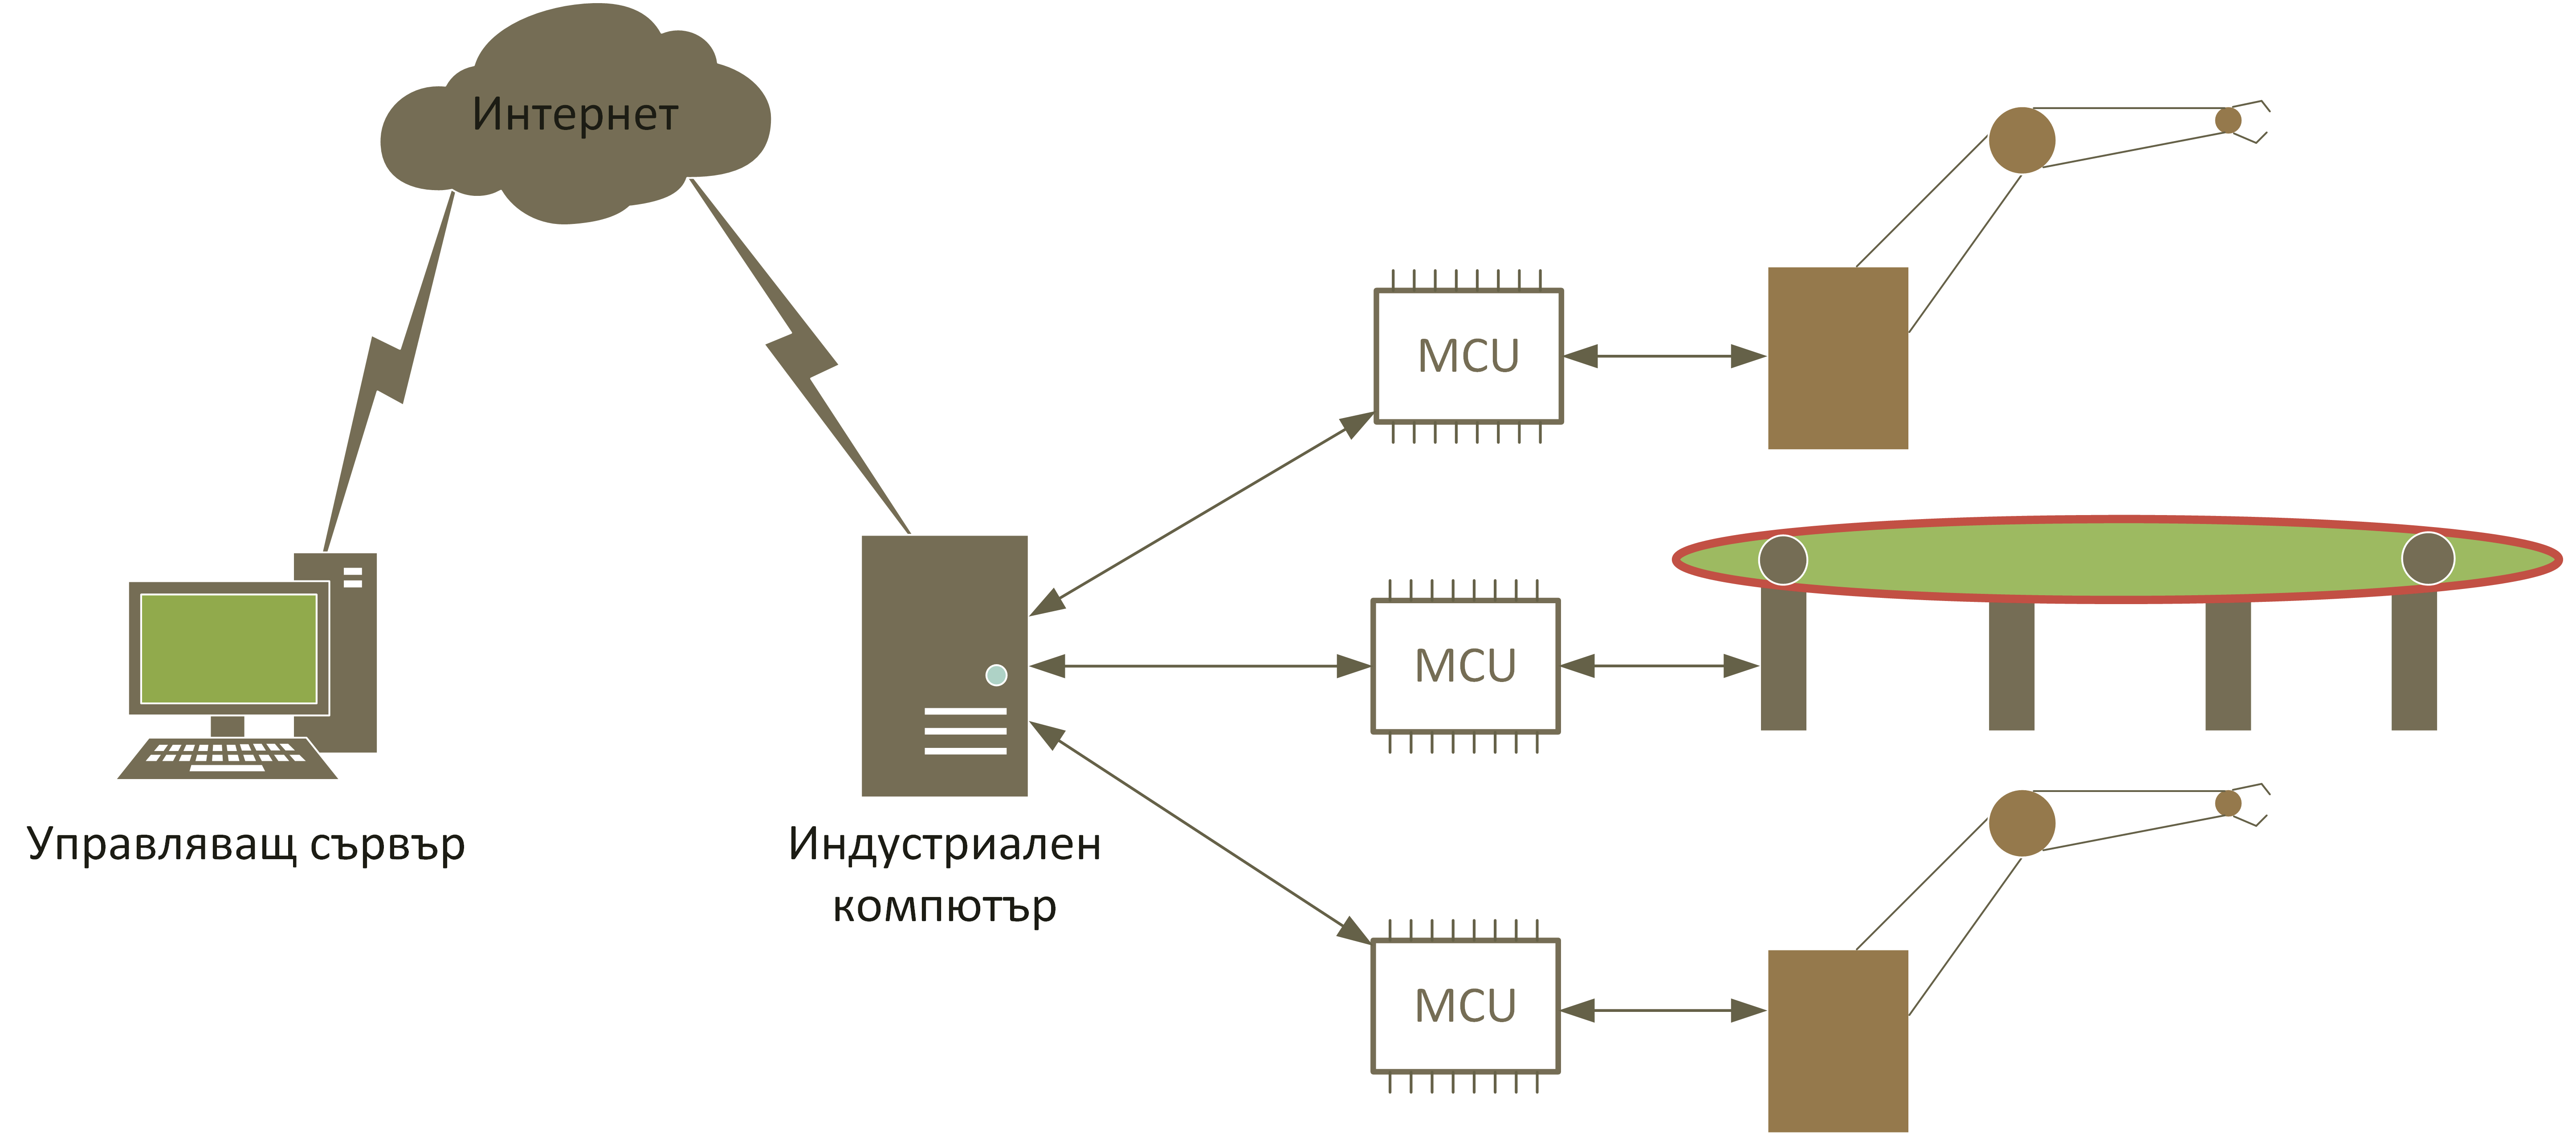
\includegraphics[width=\linewidth]{pictures/ROBKO_example_use.png}
    \caption{Пример за отдалечено управление на поточна линия}
    \label{fig:example_use}
\end{figure}
\chapter{Система за автоматизирано отдалечено управление на РОБКО 01 с
възможност за ръчен контрол}
%използвани технологии
\section{Функционални изисквания}
Към настоящата разработка са поставени следните изисквания:
\begin{itemize}
    \item ръчно управление на РОБКО 01
    \item управление на робота чрез текстови команди
    \item подаване на команди през интернет
    \item четене на команди от файл
    \item опашка за команди
    \item едновременно движение на всички мотори
    \item засичане на предмет в щипката на робота
\end{itemize}
\section{Топология на системата}
На фигура \ref{fig:system} е показана блокова схема на проектираната система. Жълтите стрелки обозначават информационни сигнали, а кафявите - захранващи напрежения и токове.\\
\indent{}
Основната платка реализира връзките между отделните компоненти на системата. Прякото управление на робота се извършва от микроконтролер STM32L476RG, разположен на собствена платка. Микроконтролерът получава информация относно какви движения трябва да изпълни роботът от два източника: два джойстика (ръчно управление) и компютър в интернет, наричан клиент. Клиентът изпраща команди през интернет до втори компютър - сървъра. Сървърът е свързан с микроконтролера и препраща командите към него.\\
\indent{}
\begin{figure}[!htbp]
    \centering
    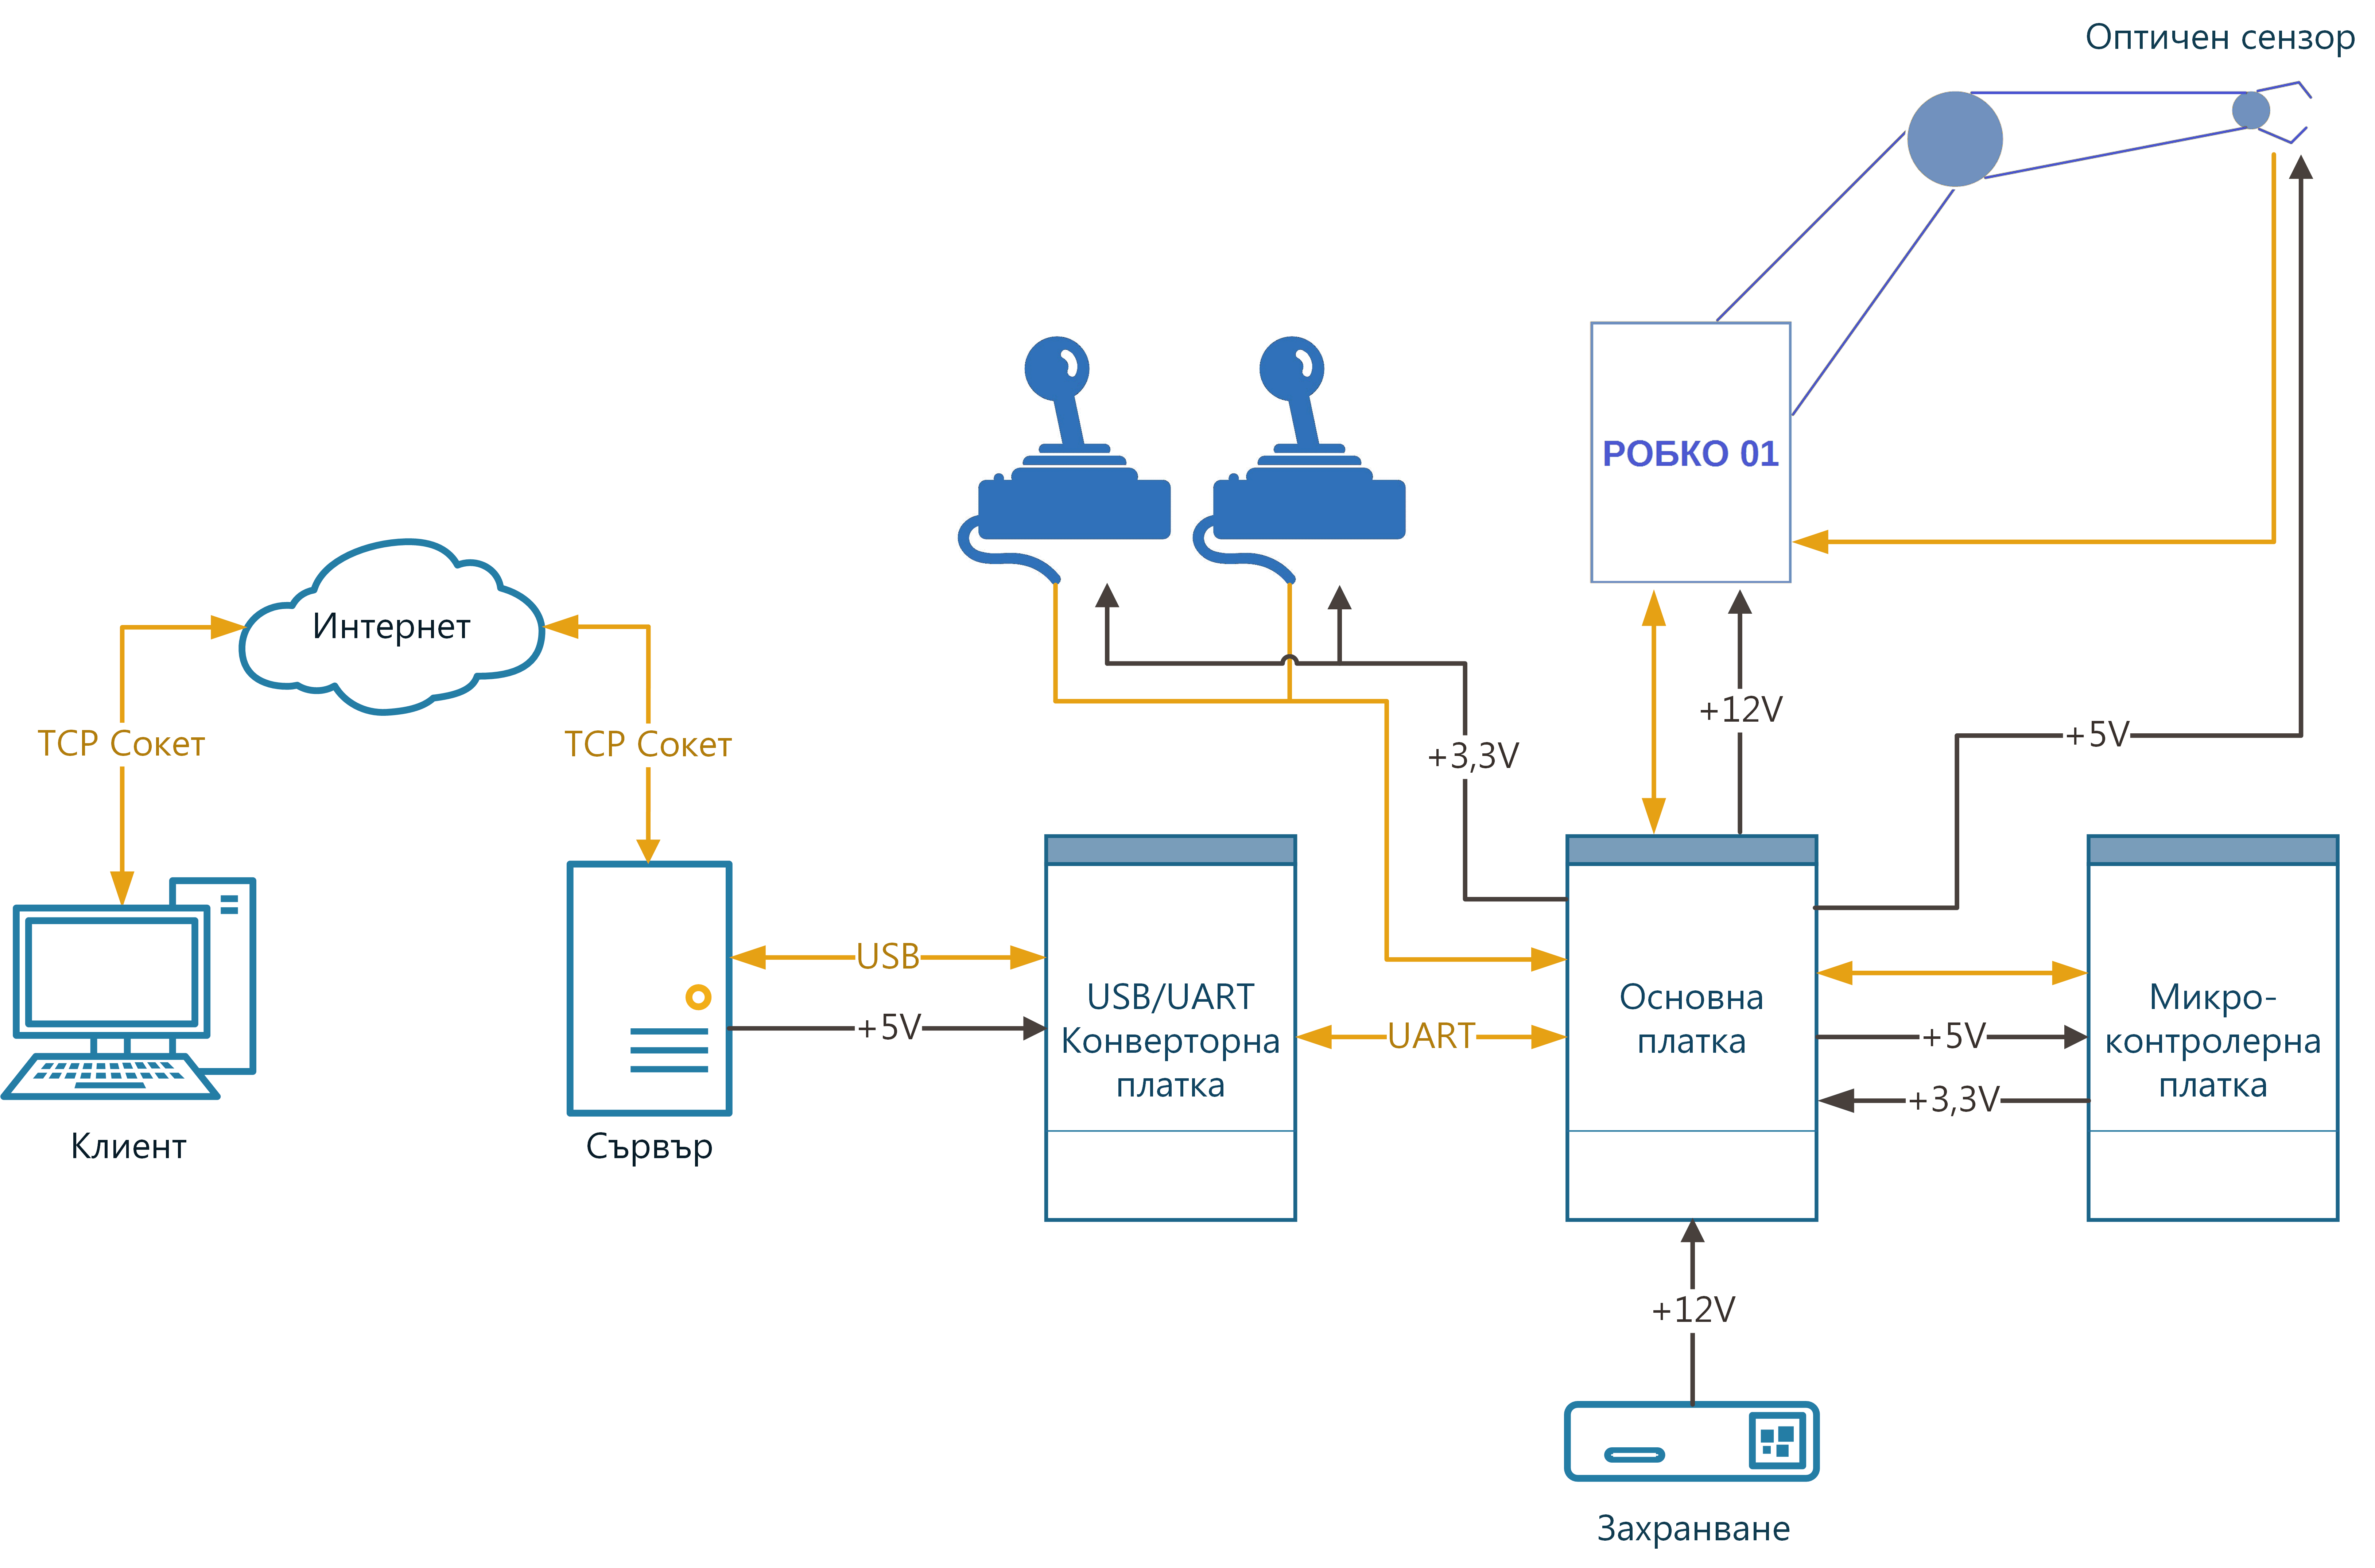
\includegraphics[angle=90,origin=center,width=\linewidth]{pictures/robko_system_diagram.png}
    \caption{Блокова схема на системата}
    \label{fig:system}
\end{figure}
\section{Компоненти на системата}
\subsection{РОБКО 01}
\subsubsection{Механика}
\indent{}
РОБКО 01 е антропоиден робот със шест степени на свобода, реализирани с кинематични връзки.
\cite{robko-man}
Изграден е от неподвижна основа, три звена и хващач. Задвижва се от шест стъпкови електромотора, означени с 5 на фигура \ref{fig:mech}. Те са монтирани от външната страна на първото звено(1). Във вътрешността му се помещават шест зъбни редуктора(6). Движението на моторите се предава към звената и щипката(4) чрез метални въжета и ролки(7).\\
\indent{}
Първото звено се върти около ос, перпендикулярна на основата. Второто(2) и третото(3) звено, наричани съответно рамо и лакът, се накланят съответно напред-назад и нагоре-надолу. Хващачът се върти и накланя нагоре-надолу. Тези движения се реализират посредством диференциална зъбна предавка, разположена между третото звено и хващача. Тя се задвижва от два мотора. При съпосочно въртене на моторите хващачът се накланя в съответната посока. Когато двата мотора се въртят противопосочно, едната страна на хващача се накланя нагоре, а другата надолу. Резултатното движение е въртене.\\
\indent{}
Върху второто звено е монтиран прекъсвач, който се затваря когато металното въже, затварящо хващача, се обтегне достатъчно. Това позволява да се засича дали хващачът е стиснал предмет. Тази функционалност не се използва в текущата разработка заради голямата сила, нужна за да се затвори прекъсвача, и опасността въжето да се скъса.
\FloatBarrier
\begin{figure}[!htb]
    \centering
    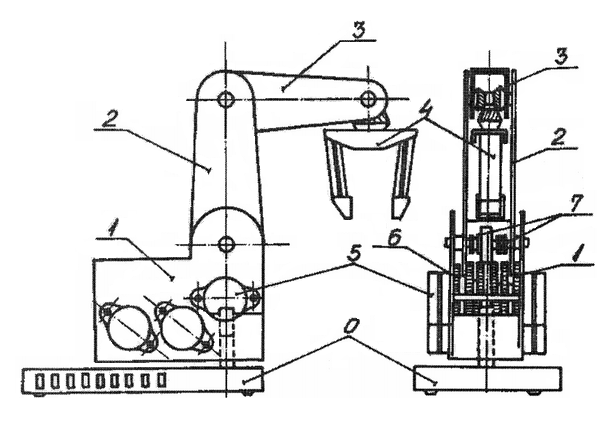
\includegraphics[width=\linewidth]{pictures/Robko_axis.PNG}
    \caption{РОБКО 01 - схема на механиката}
    \label{fig:mech}
\end{figure}
\subsubsection{Драйверна платка}
\indent{}
Драйверната платка на РОБКО 01 е описана подробно в ръководството за експлоатация
\cite{robko-man}, но липсват важни подробности. Не е обозначено кой сигнал на кой пин на конекторите е изведен. Липсват стойностите на пасивните елементи. Пропуснати са четири кондензатора. Не са дадени моделите на компонентите.\\
\indent{}
След анализ на печатната платка и с помощта на информация от интернет и от предишния собственик на робота, принципната електрическа схема на РОБКО 01 беше въстановена и попълнена с липсващата информация. На следващите страници е дадена въстановената принципна електрическа схема. Схемните страници от 10-та до 14-та включително са идентични на 9-та схемна страница и не са показани.

Цифровата логика на схемата е реализирана с ИС от серията 74LSxx и техни еквиваленти. Интегралните схеми се захранват от линеен регулатор на напрежение MA7805. На моторите и на регулатора се подава напрежение 12V.
\includepdf[pages={4},angle=90]{documents/schematic_bw.pdf}
\includepdf[pages={8-9},angle=90]{documents/schematic_bw.pdf}
\includepdf[pages={15-17},angle=90]{documents/schematic_bw.pdf}
Стъпковите електромотори са двуфазни униполярни. Двете фази са изградени от по две статорни намотки. Шестте мотора се управляват от транзисторни крайни стъпала с диодна защита от обратно напрежение. За всеки мотор отговаря по един 4-битов регистър, съхраняващ състоянията на намотките/фазите му. Чрез записване на данни в регистрите се контролира през кои намотки на стъпковите мотори да протича ток.\\
\indent{}
Не всяка от 16-те възможни стойности на регистрите съответства на позволено състояние на моторите. Непозволените комбинации се предотвратяват от логически елементи ИЛИ-НЕ. В таблица \ref{tab:step_order} са дадени позволените комбинации от токове през намотките на моторите. Индексите на токовете съответстват на индексите на битовете в регистрите за съответните мотори. За въртене в режим на полустъпка се изпълняват в дадения ред, а за режим на цяла стъпка се пропускат  полустъпките при които протича ток само през една намотка.
\begin{table}[!htb]
    \centering
    \begin{tabular}{|c|c|c|c|}
        \hline
        I$_0$ & I$_1$ & I$_2$ & I$_3$\\
        \hline
        1 & 0 & 0 & 0\\
        \hline
        1 & 0 & 1 & 0\\
        \hline
        0 & 0 & 1 & 0\\
        \hline
        0 & 1 & 1 & 0\\
        \hline
        0 & 1 & 0 & 0\\
        \hline
        0 & 1 & 0 & 1\\
        \hline
        0 & 0 & 0 & 1\\
        \hline
        1 & 0 & 0 & 1\\
        \hline
    \end{tabular}
    \captionsetup{width=0.65\linewidth}
    \caption{Поредност на стъпките на моторите за въртене в режим на полустъпка}
    \label{tab:step_order}
\end{table}
\captionsetup{width=\linewidth}
\\
\indent{}
Два допълнителни регистъра са заделени за осемте изходни пина на платката (OUT0-OUT7). Към изходите на тези регистри са свързани буфери с изходи от тип отворен колектор. Това позволява от изходните пинове на робота да се управляват товари, работещи на по-високо напрежение от ТТЛ интегралните схеми.\\
\indent{}
РОБКО 01 разполага и с осем входни пина (IN0-IN7). Данните от тях се буферират в повторители с високоимпедансно изходно състояние.

Достъпът до регистрите се контролира от 3-битов дешифратор, обуславящ 8 адреса. Първите шест адреса се отнасят за регистрите на стъпковите мотори. Последните два адреса отговарят едновременно за 8-те изходни пина и за 8-те входни пина.\\
\indent{}
Понеже РОБКО 01 е проектиран да се управлява от 8-битовия Правец 82, разполага с 8-битова
\footnote{Адресната магистрала на Правец 82 е 16-битова.
\cite{pravets82}
Разширителната платка, показана на фигура \ref{fig:orig_cntrl}, свързва РОБКО 01 с Правец 82 и транслира адресното пространство на робота в това на компютъра.}
адресна магистрала (A0-A7) и 8-битова магистрала за данни (D0-D7). Младшите
\footnote{При Правец 82 и РОБКО 01 нулевият бит е най-младши.}
4 бита от магистралата за данни се използват от компютъра (или микроконтролера) за да записва данни в регистрите на робота. Старшите четири бита се използват за четене на входните пинове на РОБКО 01.\\
\indent{}
С трите най-младши адресни бита се избира регистър или входящ буфер, а останалите адресни битове транслират тези адреси в адресното пространство на Правец 82. Те се свързват към логически елементи И-НЕ и ИЛИ-НЕ, които подават разрешаващ сигнал на дешифратора само ако старшите адресни битове имат правилните стойности. В таблица \ref{tab:addr_space} е описано адресното пространство на РОБКО 01. За права посока се приема реда на стъпки даден в таблица \ref{tab:step_order}, изпълняван от горе надолу.\\
\begin{table}[!htb]
    \centering
    \begin{tabular}{|c|c|c|}
        \hline
        Адрес & Мотор / буфер & Движение в права посока\\
        \hline
        0x98 & 0 - Ос на основата & Въртене наляво\\
        0x99 & 1 - Раменна става & Накланяне напред\\
        0x9A & 2 - Лакътна става & Повдигане нагоре\\
        0x9B & 3 - Щипка - диф. предавка, десен & Накланяне надолу\\
        0x9C & 4 - Щипка - диф. предавка, ляв & Накланяне нагоре\\
        0x9D & 5 - Щипка - пръсти & Отваряне\\
        \cline{3-3}
        0x9E & Младши входни/изходни битове & \multicolumn{1}{c}{}\\
        0x9F & Старши входни/изходни битове & \multicolumn{1}{c}{}\\
        \cline{1-2}
    \end{tabular}
    \caption{Адресно пространство на РОБКО 01}
    \label{tab:addr_space}
\end{table}
\indent{}
\FloatBarrier
РОБКО 01 има четири контролни сигнала - \textoverline{BS}, \textoverline{DINE}, \textoverline{I/O R} и \textoverline{I/O W}. Първите два не се използват.\\
\indent{}
\textoverline{I/O R} е разрешаващ сигнал за четене. Когато е в активно ниско ниво, входящите буфери подават на D4-D7 състоянията на избраните входни пинове. Когато е в неактивно ниво или е избран адрес, различен от този на входно/изходните буфери, изходите на входните буфери се намират във високоимпедансно състояние.\\
\indent{}
\textoverline{I/O W} е разрешаващ сигнал за записване. При преминаването му от неактивно в активно ниво данните, подадени на D0-D3, се записват в регистъра, чийто адрес е избран.

РОБКО 01 разполага с четири конектора. Вътрешният конектор се свързва към стъпковите електромотори и сензора за затваряне на щипката. На конекторът, маркиран като порт А са изведени входните и изходните пинове. Порт B е предназначен за връзка с компютър и на него са изведени адресната магистрала, магистралата за данни и контролните сигнали. Между тези два конектора се намира захранващия конектор. Изискванията към захранването са постоянно напрежение 12V ±0,6V и максимален ток 5A.
\cite{robko-man}
\subsubsection{Оптичен сензорен хващач}
\label{opto_claw_section}
\indent{}
От трите накрайника на РОБКО 01 се използва оптичния сензорен хващач. Представлява щипка с монтирани инфрачервен светодиод на единия "пръст", фототранзистор на другия и малка печатна платка върху тялото (виж фигура \ref{fig:robko_opto}).\\
\indent{}
На следващата страница е показана принципната електрическа схема на оптичния сензорен хващач. Такава схема не присъства в ръководството за експлоатация на РОБКО 01
\cite{robko-man}, не е налична и в интернет. Показаната схема е изработена след анализ на печатната платка на хващача.\\
\indent{}
D9 е инфрачервеният светодиод, който осветява фототранзистора Q3. Q3 работи в активен режим и пропуска достатъчно ток през базата на Q2 за да го отпуши. Входът на U3:B попада във високо ниво и изходът му преминава в ниско. В следствие на това изходите на U3:A и U3:C преминават във високо ниво. D8 не свети, изходът на U3:D е в ниско ниво. Пинове 3 и 5 на конектор J29 са съответно във високо и ниско ниво.\\
\indent{}
Когато предмет попадне между "пръстите" на щипката, светлинния лъч от D9 се препречва. Транзисторите Q3 и Q2 се запушват и четирите логически елемента сменят състоянията на изходите си. D8 започва да свети, а пиновете 3 и 5 на J29 разменят състоянията си (3-ти преминава в ниско, 5-ти във високо).\\
\indent{}
Пин 5 на конектор J29 се свързва към пин 33 (IN6) на порт A на РОБКО 01. Това позволява на микроконтролера да чете състоянието му през регистрите на драйверната платка. Пинове 1 и 2 се свързват съответно към пинове 2 и 1 на конектор J23 на основната платка, откъдето се захранва оптичния сензорен хващач. Причината хващачът да не се захранва от драйверната платка е, че на портовете на робота не е изведено +5V захранващо напрежение и всички изходни пинове са от тип отворен колектор.
\includepdf[pages={5},angle=90]{documents/schematic_bw.pdf}
%принципна електрическа схема (в приложение?)
%електрически параметри
\subsection{STM32L476RG Nucleo}
Системата за управление на РОБКО 01 се базира на микроконтролерната платка STM32L476RG Nucleo, показана на фигура \ref{fig:nucleo}. Платките от серията Nucleo на ST Microelectronics комбинират микроконтролер, програматор, дебъгер и помощни елементи (светодиоди, прекъсвачи и конектори).\cite{nucleo_man} Програматор/дебъгерът е втори, по-малък микроконтролер. Намира се в горната част на платката.\\
\indent{}
Използваният микроконтролер - 32-битовият STM32L476RG разполага с ARM ядро с вграден FPU (Floating Point Unit). Отличава се със свръхниска консумация - 30nA в най-маломощен режим. Ядрото поддържа прекъсвания и работи с максимална тактова честота 80MHz. Микроконтролерът разполага с 1MB флаш памет и 128KB статична RAM памет. Има DMA (Direct Memory Access) блок. Съдържа множество периферни модули - UART, SPI, I2C, LCD драйвер, 12-битови АЦП и ЦАП, таймери и други.
\cite{mcu_specs}\\
\indent{}
\begin{figure}[!thb]
    \centering
    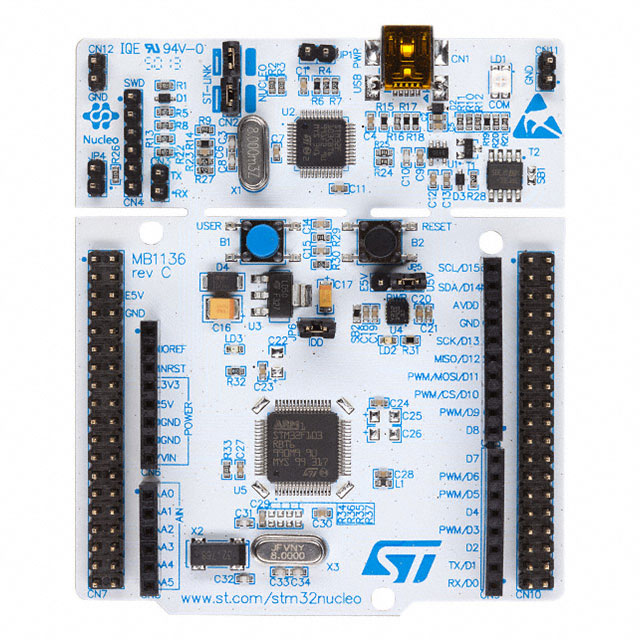
\includegraphics[width=0.85\linewidth]{pictures/nucleo_board.jpg}
    \caption{Микроконтролерна платка STM32L476RG Nucleo}
    %Да, ама не! Това е STM32F103
    \label{fig:nucleo}
\end{figure}
\FloatBarrier
Микроконтролерът се свързва с адресната магистрала, магистралата за данни и контролните сигнали на РОБКО 01. Това му позволява да чете и пише в регистрите на драйверната платка. Софтуерът на микроконтролера се разглежда подробно в глава \ref{firmware_chapter}. Основната му функция е да определя какви стойности да записва в регистрите на драйверната платка на РОБКО 01 за да бъдат изпълнени желаните движения.
\subsection{Основна платка и адаптери}
В рамките на настоящата разработка са проектирани и изработени три печатни платки. Две от тях са пасивни адаптери за специфичните конектори на РОБКО 01. Печатната платка означена на фигура \ref{fig:system} като "Основна платка" служи за централен възел на системата - свързва отделните модули един към друг. Също така предоставя визуална индикация за състоянието на моторите, възможност за настройка и петволтово захранване. Проектираните печатни платки се разглеждат подробно в глава \ref{boards_chapter}.
\subsection{USB/UART модул}
Комуникацията между сървърният компютър и микроконтролера се извършва по серийна UART връзка. Скоростта е 115200 бода, изпращат се осембитови думи с по един допълнителен бит за проверка по четност и предаването на данни се завършва с един стоп бит. Битът за проверка по четност е единица, когато в осемте бита на предаваната дума има четен брой единици. Връзката между микроконтролера и компютъра преминава през USB/UART адаптерна платка, показана на фигура \ref{fig:usb_uart}. Сървърният софтуер достъпва USB/UART модула като виртуален сериен порт, свързан по USB връзка.
\begin{figure}[!htb]
    \centering
    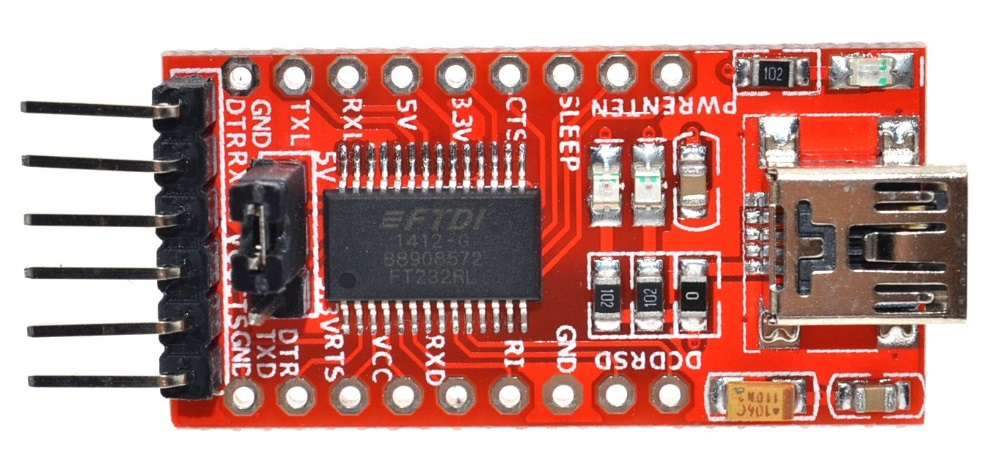
\includegraphics[width=0.75\linewidth]{pictures/USB_to_UART.jpg}
    \caption{USB/UART адаптерна платка}
    \label{fig:usb_uart}
\end{figure}
\FloatBarrier
\subsection{Компютри и софтуер за отдалечено управление}
Отдалеченото управление през Интернет се реализира чрез две програми - клиент и сървър. Клиентската програма чете текстови команди, въвеждани от потребителя в команден ред и ги изпраща през TCP сокет към сървърната програма. На сървъра се съхраняват файлове, съдържащи предварително въведени поредици от команди. Сървърната програма препраща получените команди към микроконтролера или прочита файл и изпраща записаните в него команди. Двете програми и форматът на командите се описват в глава \ref{network_chapter}.\\
\indent{}
За реализацията на проекта един и същи компютър е използван и като клиент, и като сървър. Клиентската програма се изпълнява на виртуална машина Ubuntu Server. Употребата на виртуална машина позволява клиентската и сървърната програма да използват различни IP адреси, което е наложително за тестване на мрежовата свързаност.\\
\indent{}
При имплементация на подобна система в промишлени условия сървърният компютър вероятно ще бъде индустриален, а клиентският - обикновен персонален компютър. Индустриалните компютри се отличават с по-високи изисквания за издръжливост на температура, прах, механични вибрации и удари, електромагнитни смущения и влага. Често разполагат със специализирани конектори и са предназначени за монтаж в табла, на стени или в шкафове.
%източник?
\subsection{Джойстици}
\label{joysticks}
Ръчното управление на робота се осъществява посредством два джойстика, показани на фигура \ref{fig:joysticks}. Разполагат с по два бутона и една дръжка. Джойстиците са произведени като периферни устройства за Правец 8\cite{joystick_pravets} и са директно копие на джойстик A2M2002, произвеждан от Apple.\cite{joystick_apple} Движението на дръжката завърта два потенциометъра. Измерването на съпротивлението им се е извършвало с помощта на таймер 558, свързан като чакащ мултивибратор. Продължителността на генерираните от таймера импулси е пропорционална на съпротивлението и съответно на позицията на дръжката на джойстика.
\cite{joystick_explained}\\
\indent{}
\begin{figure}[!htb]
    \centering
    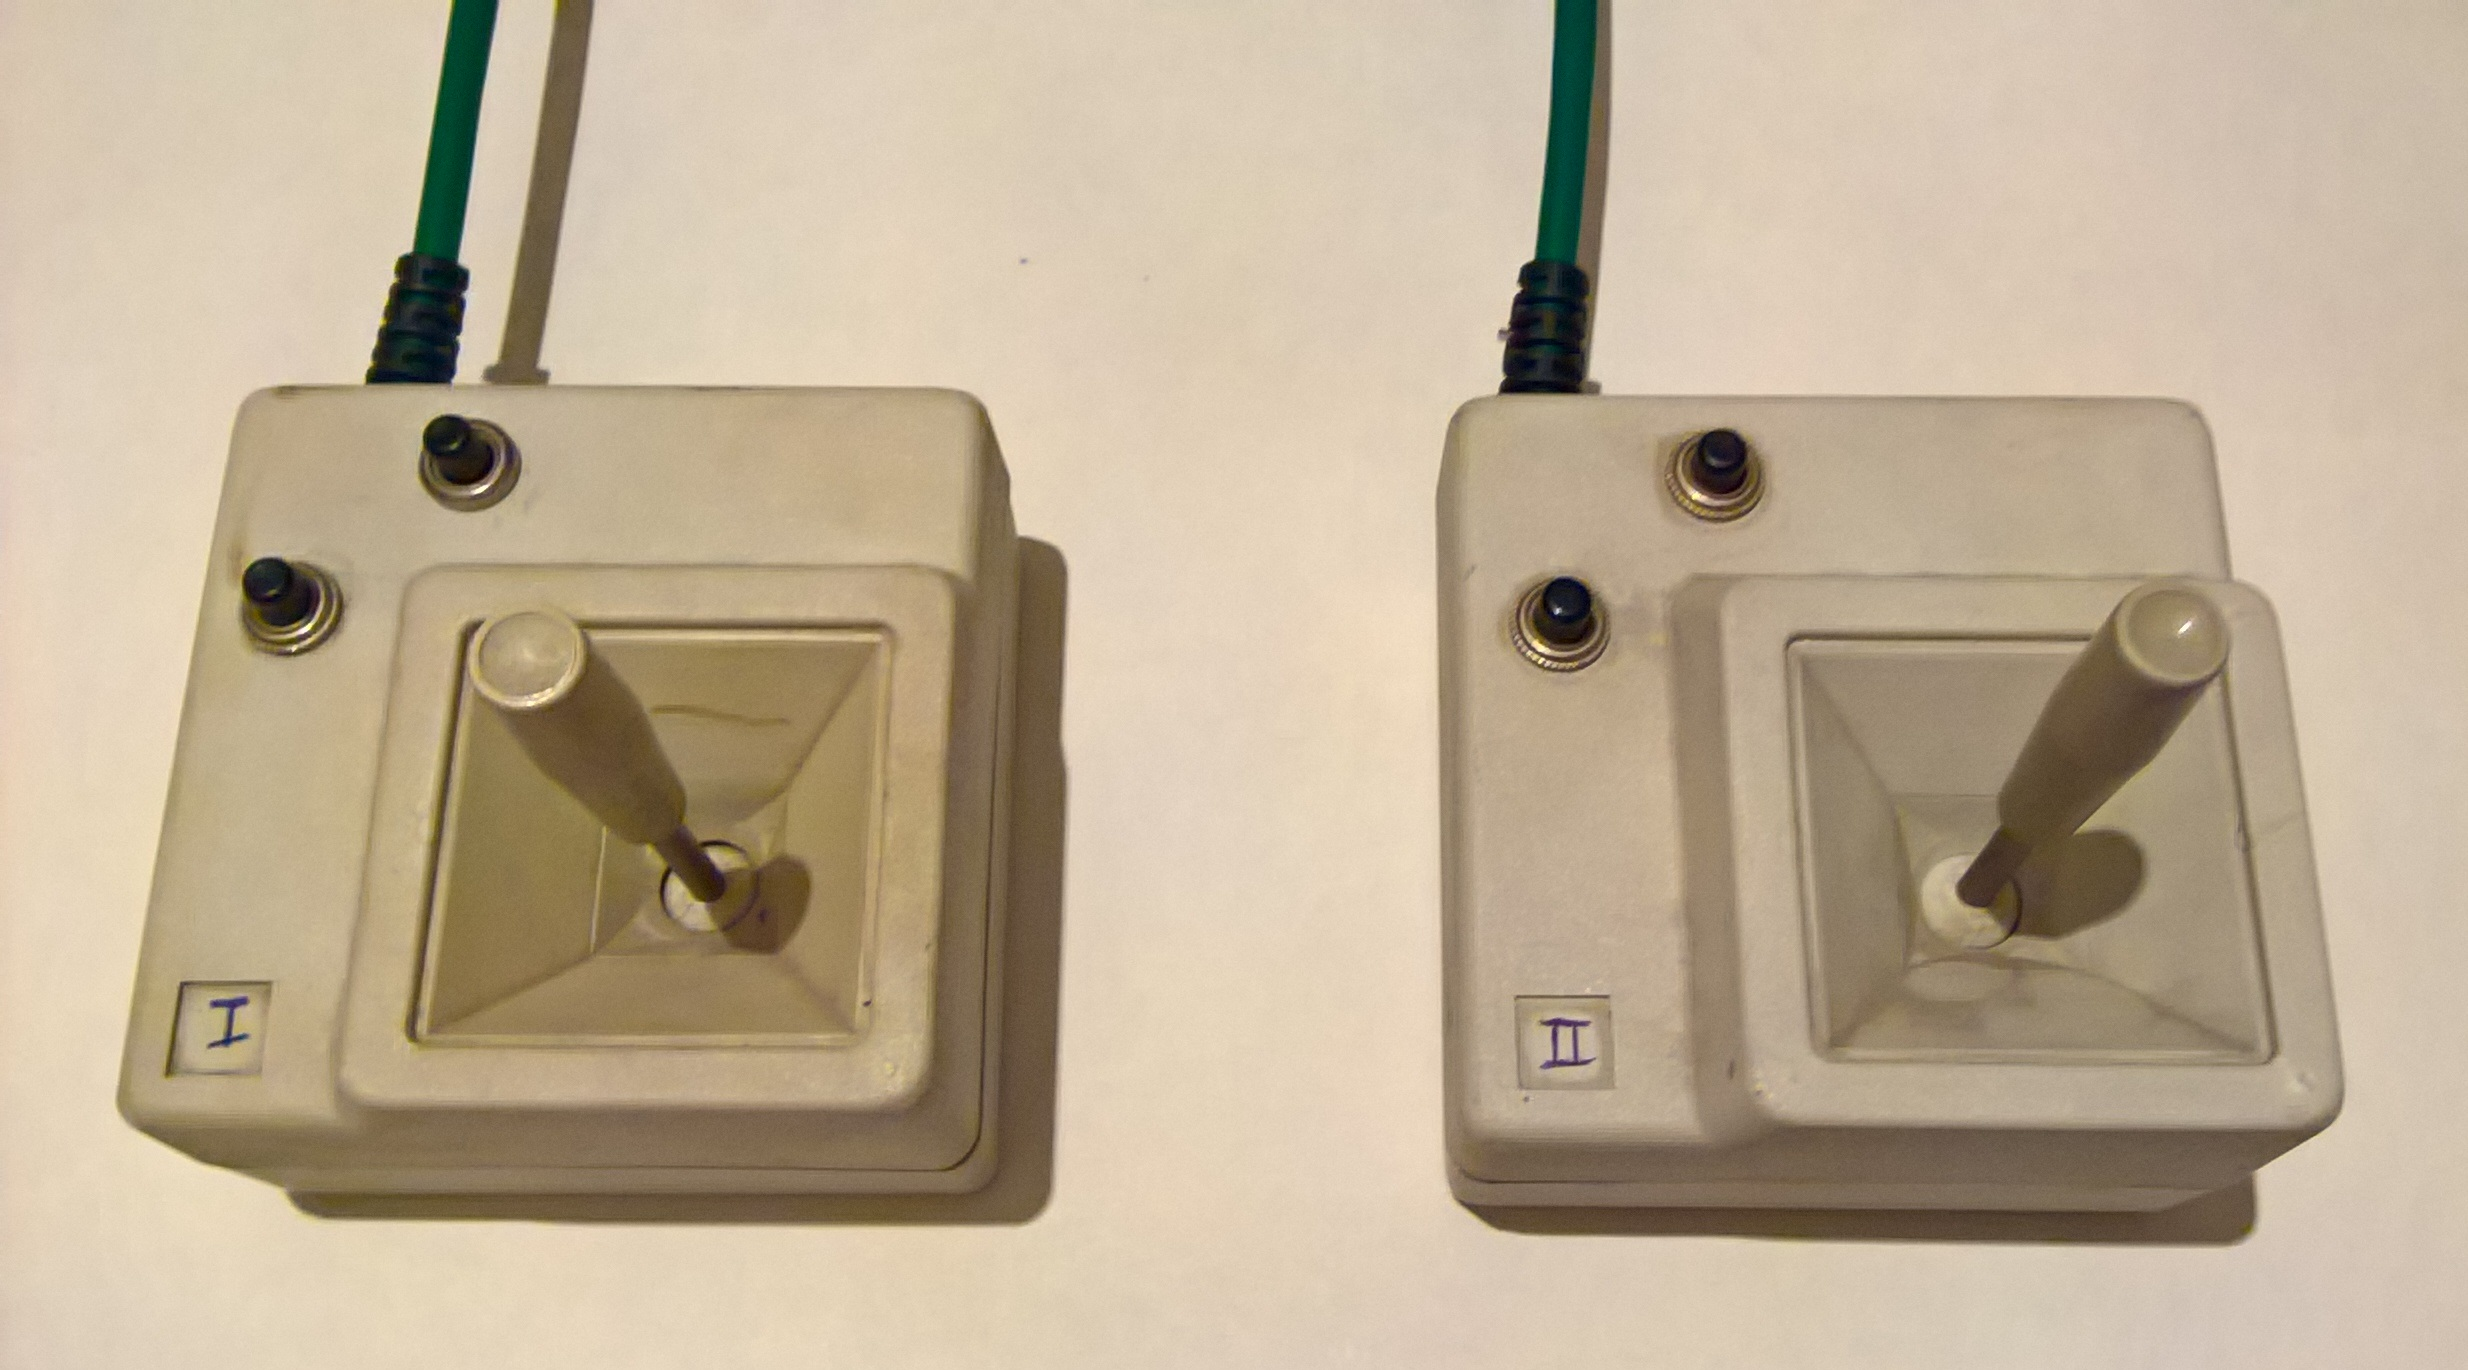
\includegraphics[width=\linewidth]{pictures/joysticks.jpg}
    \caption{Модифицирани джойстици за Правец 8}
    \label{fig:joysticks}
\end{figure}
За да се използват в настоящата разработка двата джойстика са модифицирани. Оригиналните им кабели са заменени с UTP Cat 5 кабели с накрайници RJ45. Неизползваните изводи на потенциометрите са свързани към захранващото напрежение, образувайки делител на напрежение. На следващата страница е показана принципната електрическа схема на джойстиците след извършените модификации. Първите два пина се използват за засичане на джойстиците от микроконтролера. Когато и двата джойстика са свързани към основната платка, през тези окъсени пинове се изгражда връзка между пин PC7 на микроконтролера и 3,3V захранване.\\
\indent{}
Първият джойстик се свързва към конектор RJ1 на основната платка, а вторият към RJ2 (виж точка \ref{manual_cntrl_section}). За горна страна се приема страната, от която излиза кабелът. В таблица \ref{tab:joysticks} се описва кой джойстик се използва за управлението на какви движения на РОБКО 01.
\begin{table}[!th]
    \centering
    \begin{tabular}{|c|c|c|}
        \hline
        Джойстик & Позиция/натиснат бутон & Движение на РОБКО 01\\
        \hline
        \multirow{6}{*}{Първи} & дръжка наляво & щипка - въртене наляво\\
        & дръжка надясно & щипка - въртене надясно\\
        \cline{2-3}
        & дръжка нагоре & повдигане лакът\\
        & дръжка надолу & сваляне лакът\\
        \cline{2-3}
        & горен бутон & щипка - завъртане нагоре\\
        & долен бутон & щипка - завъртане надолу\\
        \hline
        \multirow{6}{*}{Втори} & дръжка наляво & основа - въртене наляво\\
        & дръжка надясно & основа - въртене надясно\\
        \cline{2-3}
        & дръжка нагоре & рамо назад\\
        & дръжка надолу & рамо напред\\
        \cline{2-3}
        & горен бутон & щипка - стискане\\
        & долен бутон & щипка - отпускане\\
        \hline
    \end{tabular}
    \caption{Съответствия между джойстици и движения на РОБКО 01}
    \label{tab:joysticks}
\end{table}
\FloatBarrier
\includepdf[pages={6},angle=90]{documents/schematic_bw.pdf}
\subsection{Захранване}
Системата се захранва от 12-волтово импулсно захранване\footnote{с изключение на двата компютъра и USB/UART конверторната платка, която се захранва от сървърния компютър, виж фиг. \ref{fig:system}}, показано на фигура \ref{fig:psu}. Максималният изходен ток на захранването е 10A, максималната мощност е 120W. Според спецификациите на импулсното захранване входното му напрежение е в обхвата от 110V до 220V, но функционира правилно и при входно напрежение 230V.
\begin{figure}[!htb]
    \centering
    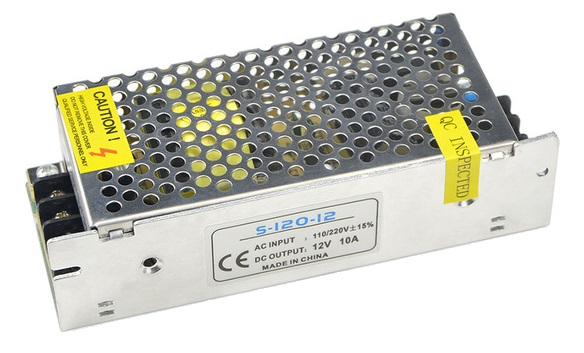
\includegraphics[width=0.8\linewidth]{pictures/PSU.jpg}
    \caption{Захранващ източник}
    \label{fig:psu}
\end{figure}
\chapter{Проектирани печатни платки}
\label{boards_chapter}
%\section{Функции и параметри}  %явява се повторение
%адаптер
%индикация
%захранване
\section{Принципна електрическа схема}
\subsection{PATA адаптер и тестов адаптер}
Тестовият адаптер свързва оригиналният кабел на РОБКО 01 с микроконтролерната платка. Отделните проводници от кабела са запоени адаптерната платка и са свързани към стандартен двуредов конектор. Сигналите \textoverline{DINE} и \textoverline{BS} не са изведени, а сигналите A4-A7 се свързват към външни установяващи съпротивления върху прототипна платка. Този адаптер е използван само за тестване на разработката преди да бъдат произведени другите две платки.

Серията РОБКО разполага със собствен специфичен конектор. Броят пинове на този конектор и на стандартния PATA конектор съвпадат. Това позволява РОБКО 01 да се свързва към управляващо устройство през стандартен PATA лентов кабел с подходящ адаптер. Това е функцията на втората платка от настоящата система. Всеки проводник от РОБКО конектора е свързан със съответен проводник от PATA конектора. Изключение прави средният ред на РОБКО конектора. Тези проводници са свързани заедно и към същия брой пинове в PATA конектора. В различните портове на РОБКО 01 те са свързани или към земя или към захранване, но винаги всички заедно.\\
\indent{}
РОБКО/PATA адаптерът е двустранна платка. От едната страна е PATA конекторът, а от другата РОБКО конекторът или три стандартни едноредови конектори. Поставя се директно в порт B на РОБКО 01. Може да се използва и за порт A на РОБКО 01.
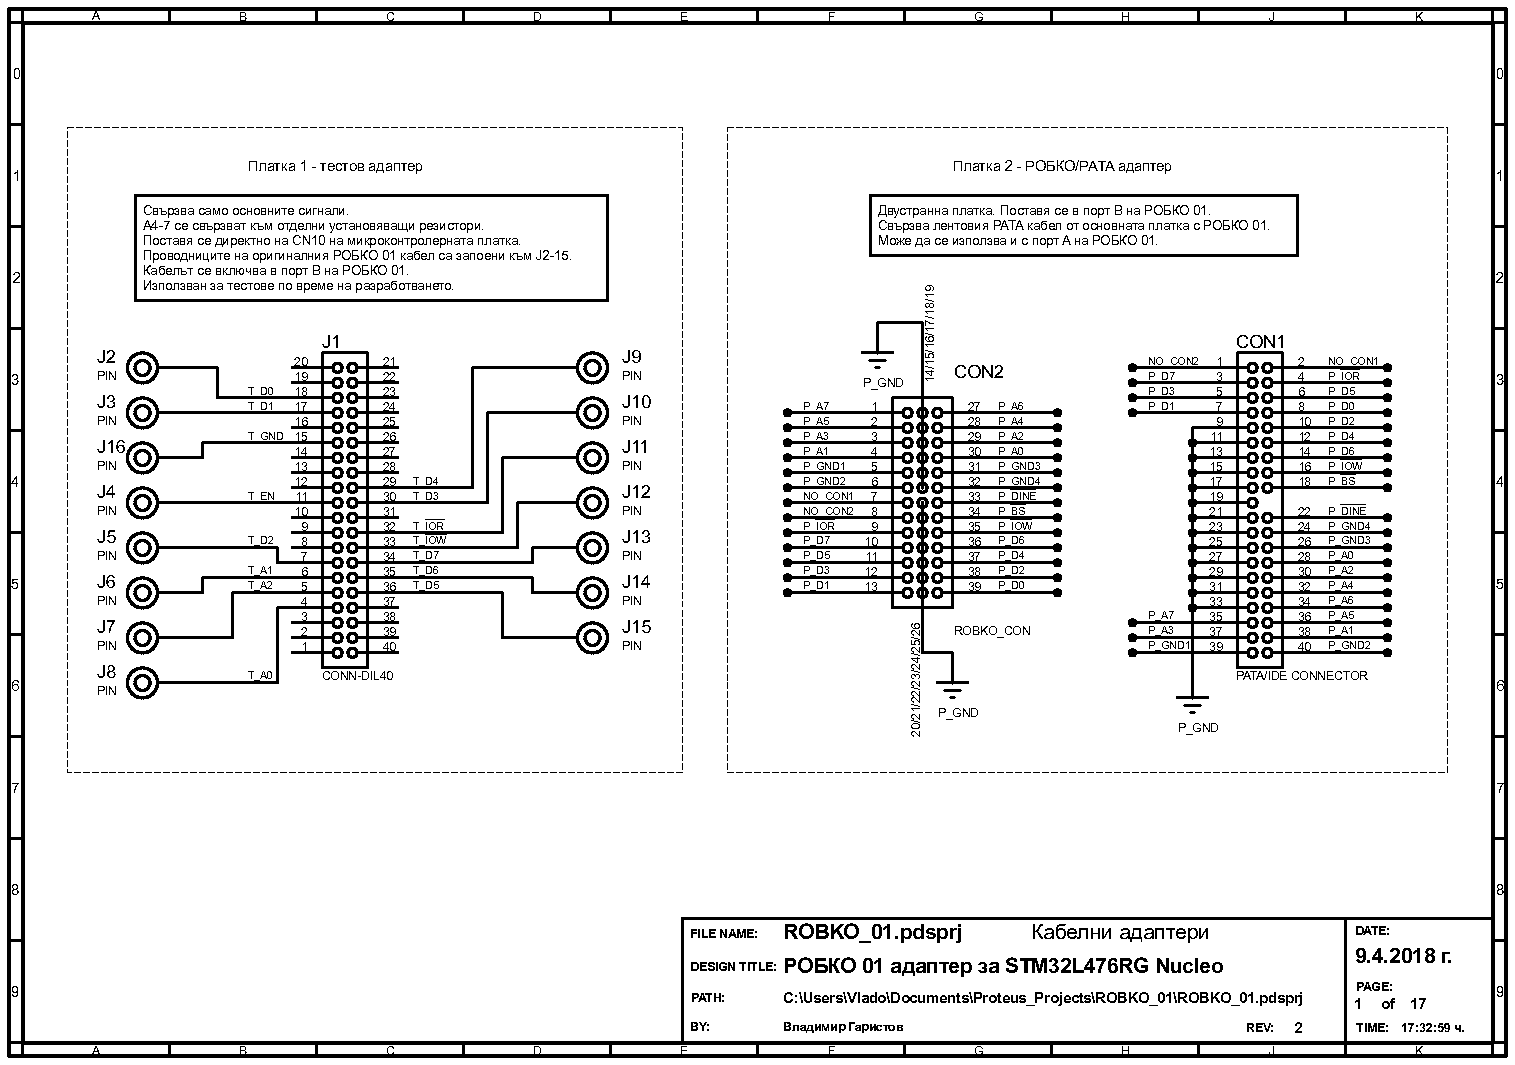
\includepdf[pages={1},angle=90]{documents/schematic_bw.pdf}
\subsection{Захранващ блок}
Захранващият блок е част от основната платка. SW3 е главният прекъсвач. През него протича захранващият ток за РОБКО 01 и за микроконтролерната платка. Схемата черпи енергия от 12-волтов източник, свързан към конектор J21. Конектор J22 подава напрежение на РОБКО 01, а конектор J23 на оптичният сензорен хващач. Микроконтролерната платка се захранва през конектор J17, показан на схемна страница "Конектори и индикация". През същия конектор основната платка получава 3,3V захранващо напрежение от линеен регулатор на микроконтролерната платка. С 3,3V се захранват джойстиците.\\
\indent{}
Захранването включва три защити - против късо съединение, против пренапрежение и против грешен поляритет на напрежението. Защитата от късо съединение се реализира с два 5-амперови бушона. Първият от тях обхваща РОБКО 01 и микроконтролерната платка, а другият само робота. Бушоните са бавнодействащи с цел да се избегне изгарянето им при кратки токови импулси, породени от индуктивния характер на моторите. Защитата против пренапрежение се осъществява чрез двупосочен трансил с номинално пробивно напрежение 13,3 V. Защитата от грешен поляритет на захранващото напрежение се реализира от P-канален MOSFET Q1, ценеров диод D7 и резистор R17. При правилен поляритет на напрежението протича ток през паразитния диод на Q1. D7 и R17 образуват делител на напрежение. Напрежението гейт-сорс на Q1 става равно на пробивното напрежение на D7 и транзисторът се отпушва. Ако на схемата се подаде отрицателно захранващо напрежение, диодът на Q1 се явява свързан в обратна посока и транзисторът остава запушен.\\
\indent{}
Микроконтролерната платка и оптичният сензорен хващач се захранват от U1 - линеен регулатор на напрежение 7805 с максимален ток 1,5A. Двете захранващи напрежения +12V и +5V се стабилизират от по един 100$\mu$F кондензатор. Монтажните отвори са заземени. През металните болтове и отстъпи те се свързват електрически с металното шаси на захранващия източник, а през него и със заземяващия проводник на сградната електроинсталация.
\includepdf[pages={3},angle=90]{documents/schematic_bw.pdf}
\subsection{Връзка между STM32L476RG и РОБКО 01}

Основната платка играе ролята на централен възел, свързващ другите компоненти на системата. Конектори CN7 и CN10 на микроконтролерната платка се свързват съответно с конектори J17 и J20 от основната. Конектори J17 и J20 се намират на страна спойки с цел микроконтролерната платка да се поставя под основната. Двете платки се прикрепят една към друга и към корпуса на захранващия източник с помощта на метални отстъпи и болтове. В конектор CON3 на основната платка се поставя единия край на лентовия PATA кабел към РОБКО 01. Резисторите R1-R4 установявят адресните сигнали A4-A7. Конектори J18 и J19 се свързват с USB-UART конверторната платка, която се свързва с компютъра изпълняващ сървърния софтуер.
\subsection{Индикация}
Светодиодите D1-D6 предоставят визуална индикация на състоянията на стъпковите мотори. Диод D1 съответства на мотор 0, D2 на мотор 1 и т.н. Номерата на моторите са обозначени на ситопечата от страна компоненти на платката и в таблица \ref{tab:addr_space}. Светодиодите са по два в корпус - зелен и червен. Зеленият цвят означава движение напред, а червеният - движение назад. При неподвижен мотор съответните светодиоди не светят.
\subsection{Ръчно управление}
\label{manual_cntrl_section}
Джойстиците за ръчно управление се описват подробно в точка \ref{joysticks}. Кабелите им се свързват към конектори RJ1 и RJ2. За определяне на ориентацията на джойстиците се използва вградения в микроконтролера аналогово-цифров преобразувател. Различните режими на управление се конфигурират от прекъсвачите SW1.\\
\indent{}
Първият прекъсвач (обозначен с единица върху корпуса на компонента; между пинове 4 и 5 на схемата) конфигурира скоростта на въртене на моторите. Когато е отворен е избрана бавна скорост, а когато е затворен - бърза. Чрез вторият прекъсвач се избира дали стъпковите мотори да се задвижват в режим на пълна стъпка (отворен) или на полустъпка (затворен). Третият прекъсвач се взима под внимание само ако четвъртият е отворен. Чрез него се избира режима на управление, като отворен съответства на отдалечено управление, а затворен на ръчно. Последният прекъсвач включва възможността на микроконтролера да засича дали двата джойстика са свързани към платката и ако са, автоматично да премине в ръчен режим.
При отворен прекъсвач тази функционалност е изключена.
%добави RPM
Бутонът SW2 рестартира микроконтролера.
\includepdf[pages={2},angle=90]{documents/schematic_bw.pdf}
\section{Графични оригинали на печатните платки}
Всички графични оригинали са в отношение 1:1 спрямо физически реализираните печатни платки.\\
Тестовият адаптер е ръчно изработен на базата на фабрично пробита и метализирана прототипна платка. Другите две печатни платки са произведени машинно.
\FloatBarrier
\subsection{Тестов адаптер}
\begin{figure}[!htbp]
    \begin{minipage}{0.49\linewidth}
        \centering
        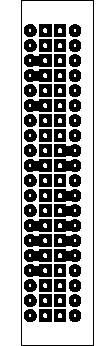
\includegraphics[page=1]{documents/dev_board.pdf}
        \caption{Страна спойки}
        \label{fig:dev_top}
    \end{minipage}
    \hfill
    \begin{minipage}{0.49\linewidth}
        \centering
        \includegraphics[page=2]{documents/dev_board.pdf}
        \caption{Страна компоненти}
        \label{fig:dev_bot}
    \end{minipage}
\end{figure}
\begin{figure}[!htbp]
    \begin{minipage}{0.49\linewidth}
        \centering
        \includegraphics[page=3]{documents/dev_board.pdf}
        \caption{Ситопечат,\\страна спойки}
        \label{fig:dev_top_silk}
    \end{minipage}
    \hfill
    \begin{minipage}{0.49\linewidth}
        \centering
        \includegraphics[page=4]{documents/dev_board.pdf}
        \caption{Ситопечат,\\страна компоненти}
        \label{fig:dev_bot_silk}
    \end{minipage}
\end{figure}
\begin{figure}[!htb]
    \begin{minipage}{0.49\linewidth}
        \centering
        \includegraphics[page=5]{documents/dev_board.pdf}
        \caption{Изолационен лак,\\страна спойки}
        \label{fig:dev_top_res}
    \end{minipage}
    \hfill
    \begin{minipage}{0.49\linewidth}
        \centering
        \includegraphics[page=6]{documents/dev_board.pdf}
        \caption{Изолационен лак,\\страна компоненти}
        \label{fig:dev_bot_res}
    \end{minipage}
\end{figure}
\begin{figure}[!htb]
    \begin{minipage}{0.49\linewidth}
        \centering
        \includegraphics[page=7]{documents/dev_board.pdf}
        \caption{Очертание\\на печатната платка}
        \label{fig:dev_cont}
    \end{minipage}
    \hfill
    \begin{minipage}{0.49\linewidth}
        \centering
        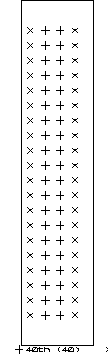
\includegraphics[page=1]{documents/dev_board_drill.pdf}
        \caption{Отвори}
        \label{fig:dev_drill}
    \end{minipage}
\end{figure}
\FloatBarrier
\subsection{PATA адаптер}
\begin{figure}[!htb]
    \begin{minipage}{0.49\linewidth}
        \centering
        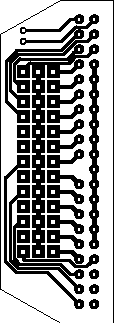
\includegraphics[page=1]{documents/pata_board.pdf}
        \caption{Страна компоненти}
        \label{fig:pata_top}
    \end{minipage}
    \hfill
    \begin{minipage}{0.49\linewidth}
        \centering
        \includegraphics[page=2]{documents/pata_board.pdf}
        \caption{Страна спойки}
        \label{fig:pata_bot}
    \end{minipage}
\end{figure}
\begin{figure}[!htbp]
    \begin{minipage}{0.49\linewidth}
        \centering
        \includegraphics[page=3]{documents/pata_board.pdf}
        \caption{Ситопечат,\\страна компоненти}
        \label{fig:pata_top_silk}
    \end{minipage}
    \hfill
    \begin{minipage}{0.49\linewidth}
        \centering
        \includegraphics[page=4]{documents/pata_board.pdf}
        \caption{Ситопечат,\\страна спойки}
        \label{fig:pata_bot_silk}
    \end{minipage}
\end{figure}
\begin{figure}[!htbp]
    \begin{minipage}{0.49\linewidth}
        \centering
        \includegraphics[page=5]{documents/pata_board.pdf}
        \caption{Изолационен лак,\\страна компоненти}
        \label{fig:pata_top_res}
    \end{minipage}
    \hfill
    \begin{minipage}{0.49\linewidth}
        \centering
        \includegraphics[page=6]{documents/pata_board.pdf}
        \caption{Изолационен лак,\\страна спойки}
        \label{fig:pata_bot_res}
    \end{minipage}
\end{figure}
\begin{figure}[!htbp]
    \begin{minipage}{0.49\linewidth}
        \centering
        \includegraphics[page=7]{documents/pata_board.pdf}
        \caption{Очертание на\\печатната платка}
        \label{fig:pata_cont}
    \end{minipage}
    \hfill
    \begin{minipage}{0.49\linewidth}
        \centering
        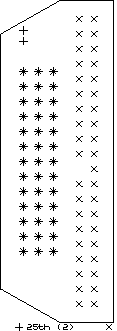
\includegraphics[page=1]{documents/pata_board_drill.pdf}
        \caption{Отвори}
        \label{fig:pata_drill}
    \end{minipage}
\end{figure}
\FloatBarrier
\subsection{Основна платка}
\begin{figure}[!htbp]
    \centering
    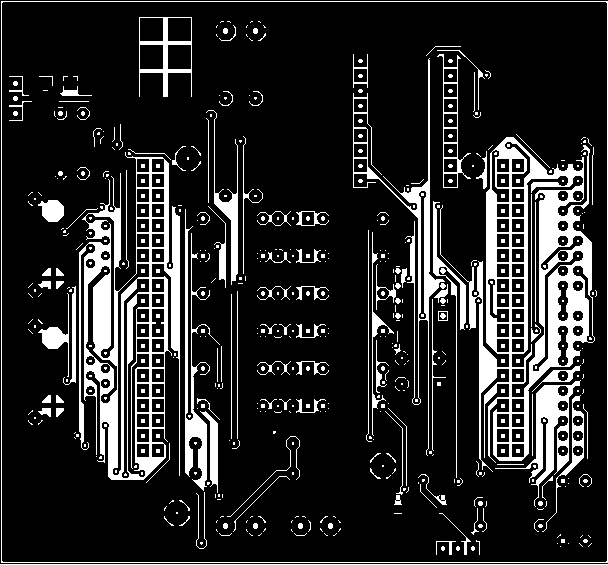
\includegraphics[page=1]{documents/main_board.pdf}
    \caption{Страна компоненти}
    \label{fig:main_top}
\end{figure}
\begin{figure}[!htbp]
    \centering
    \includegraphics[page=2]{documents/main_board.pdf}
    \caption{Страна спойки}
    \label{fig:main_bot}
\end{figure}
\begin{figure}[!htbp]
    \centering
    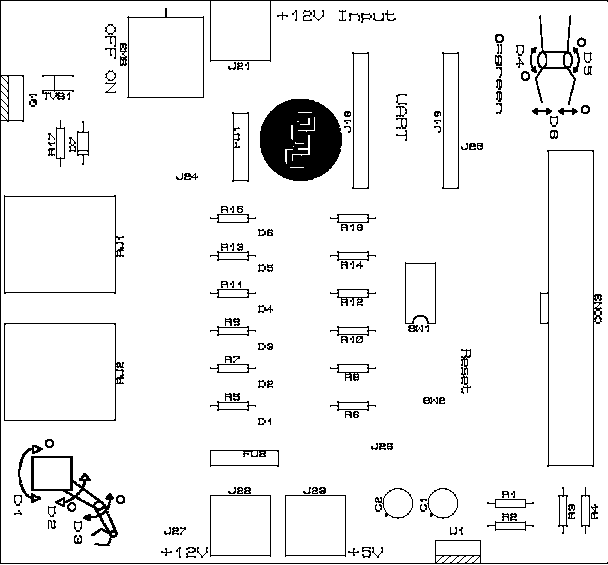
\includegraphics[page=1]{documents/top_silk.pdf}
    \caption{Ситопечат, страна компоненти}
    \label{fig:main_top_silk}
\end{figure}
\begin{figure}[!htbp]
    \centering
    \includegraphics[page=4]{documents/main_board.pdf}
    \caption{Ситопечат, страна спойки}
    \label{fig:main_bot_silk}
\end{figure}
\begin{figure}[!htbp]
    \centering
    \includegraphics[page=5]{documents/main_board.pdf}
    \caption{Изолационен лак, страна компоненти}
    \label{fig:main_top_res}
\end{figure}
\begin{figure}[!htbp]
    \centering
    \includegraphics[page=6]{documents/main_board.pdf}
    \caption{Изолационен лак, страна спойки}
    \label{fig:main_bot_res}
\end{figure}
\begin{figure}[!htbp]
    \centering
    \includegraphics[page=7]{documents/main_board.pdf}
    \caption{Припой, страна компоненти}
    \label{fig:main_top_paste}
\end{figure}
\begin{figure}[!htbp]
    \centering
    \includegraphics[page=8]{documents/main_board.pdf}
    \caption{Очертание на печатната платка}
    \label{fig:main_cont}
\end{figure}
\begin{figure}[!htbp]
    \centering
    \includegraphics[page=1]{documents/main_board_drill.pdf}
    \caption{Отвори}
    \label{fig:main_drill}
\end{figure}
\FloatBarrier
\chapter{Софтуер за отдалечено управление}
\label{network_chapter}
\section{Формат на командите за отдалечено управление}
Отдалеченото управление се извършва посредством текстовите команди, описани в таблица \ref{tab:commands}. Командите се идентифирират по номер, когато се изпращат от клиента до сървъра, и по име, когато се въвеждат от команден ред или във файл. Командите, получени от сървъра, се изпращат към микроконтролера, където се записват в опашка и изпълняват.

\indent{}
Движението на робота се задава от командите MOV и MOVE, съответно за движение на един или на множество мотори. Команда MOV приема два параметъра - номер на мотор (виж таблица \ref{tab:addr_space}) и брой стъпки, които да изпълни. Команда MOVE приема шест параметъра - брой стъпки за изпълнение от всеки мотор, в нарастващ ред на номерата на моторите. Тази команда позволява едновременното движение на повече от един мотора. Отрицателен брой стъпки се използва за движение в обратна посока (виж таблица \ref{tab:addr_space}).\\
\indent{}
Команда OFF изключва захранването на мотора, чийто номер е подаден като параметър. За изключване на всички мотори се въвежда команда OFF със стойност на параметъра 6. Използва се когато е нужно ръчно преместване на механичните части на робота. Команда FREEZE поставя робота в режим на изчакване - прекратява изпълнението на опашката от команди. Команда OPTO се използва за засичане на предмети с оптичния сензорен хващач. Когато е изпратена команда OPTO с параметър 1 и по време на изпълнението на следващата MOV или MOVE команда бъде засечен предмет се прекратява текущата команда и се преминава към следваща. Команда OPTO с параметър 2 има същото поведение, с тази разлика, че командата за движение се прекратява, когато сензорът спре да засича предмет.
%Не питай...
\begin{table}[!htb]
    \centering
    \begin{tabular}{|c|c|p{147pt}|R{12mm}R{12mm}R{12mm}|}
        \hline
        \multirow{2}{*}{\textnumero} & \multirow{2}{*}{Име} & \centering\multirow{2}{*}{Пояснение} & \multicolumn{3}{c|}{Параметри}\\
        & & & \footnotesize{8} & \multicolumn{1}{|r|}{\footnotesize{16}} & \footnotesize{24}\\
        \hline
        \multirowcell{2}[0ex][c]{1} & \multirowcell{2}[0ex][c]{MOV} & Определен мотор извършва даден брой стъпки & \multirowcell{2}[0ex][c]{мотор} & \multicolumn{2}{|c|}{\multirowcell{2}[0ex]{стъпки}}\\
        \hline
        \multirow{2}{*}{2} & \multirow{2}{*}{MOVE} & \multirowcell{2}[0ex][l]{Всички мотори извършват\\ даден брой стъпки} & \multicolumn{2}{c|}{стъпки} &\\
        & & & \multicolumn{2}{c|}{x6} &\\
        \hline
        3 & OFF & Изключва определен мотор & \multicolumn{1}{c|}{мотор} & &\\
        \hline
        \multirow{2}{*}{4} & \multirow{2}{*}{OPEN\textunderscore FILE} & Изпълнява файл, записан на сървъра & \multicolumn{3}{c|}{\multirowcell{2}[0pt][c]{име на файла\\променлива дължина}}\\
        \hline
        \multirow{2}{*}{5} & \multirow{2}{*}{GOTO\textunderscore POS} & Запазена за бъдещо & \multicolumn{2}{c|}{позиция} &\\
        & & развитие & \multicolumn{2}{c|}{x6} &\\
        \hline
        \multirowcell{2}{6} & \multirowcell{2}[0pt][l]{GET\textunderscore POS} & Запазена за бъдещо & & &\\
        & & развитие & & &\\
        \hline
        \multirowcell{3}{7} & \multirowcell{3}{KILL} & \multirowcell{3}[0pt][l]{Аварийно спиране и\\изключване на всички\\мотори} & & &\\
        & & & & &\\
        & & & & &\\
        \hline
        \multirowcell{2}{8} & \multirowcell{2}{CLEAR} & Изчистване на опашката от команди & & &\\
        \hline
        \multirowcell{2}{9} & \multirowcell{2}{FREEZE} & Спира изпълнението на команди & & &\\
        \hline
        \multirowcell{2}{10} & \multirowcell{2}{RESUME} & Възобновява изпълнението на команди & & &\\
        \hline
        \multirowcell{2}{11} & \multirowcell{2}[0pt][l]{SAVE\textunderscore POS} & Запазена за бъдещо & & &\\
        & & развитие & & &\\
        \hline
        \multirowcell{3}{12} & \multirowcell{3}{OPTO} & Прекратяване на следващата команда, при сигнал от оптичния сензор & \multicolumn{1}{c|}{\multirowcell{3}{режим}} & &\\
        \hline
        \multirowcell{2}{13} & \multirowcell{2}{SET\textunderscore STEP} & Избор на движение с цяла стъпка или с полустъпка & \multicolumn{1}{c|}{\multirowcell{2}{стъпка}} & &\\
        \hline
        \multirowcell{2}{14} & \multirowcell{2}{SET\textunderscore SPEED} & Настройка на скоростта на стъпките & \multicolumn{1}{c|}{\multirowcell{2}{време}} & &\\
        \hline
    \end{tabular}
    \captionsetup{width=0.90\linewidth}
    \caption{Команди за отдалечено управление и техните параметри}
    \label{tab:commands}
\end{table}
Командата SET\textunderscore STEP променя режима на стъпка на моторите. Единственият й параметър има три валидни стойности: 0, 1 и 2. Те означават съответно: да се използва режимът, избран от SW1 (виж \ref{manual_cntrl_section}), полустъпка и пълна стъпка. Команда SET\textunderscore SPEED задава периода от време, който се изчаква след всяка стъпка. Параметърът й е времето в милисекунди или 0 за да се използва стойността, зададена чрез SW1.\\
\indent{}
Изброените до тук команди се записват в опашка в паметта на микроконтролера и се изпълняват в реда, в който са получени. Следващите команди са приоритетни - изпълняват се веднага при получаването им.\\
\indent{}
Такава команда е KILL. Използва се за аварийно изключване на робота. Не приема параметри, прекратява изпълнението на текущата команда и изключва всички мотори. Текущата команда не се изтрива и може да бъде възобновена. Команда RESUME също е приоритетна. Тя възобновява изпълнението на команди, спряно чрез FREEZE или KILL. Команда CLEAR изтрива цялата опашка от команди, включително и текущо изпълняваната команда.\\
\indent{}
Командата OPEN\textunderscore FILE е уникална с това, че не се изпълнява от микроконтролера, а от сървъра. Като параметър приема име на файл, чието съдържание да се изпрати от сървъра към микроконтролера. Файлът трябва да съдържа команди в описания тук формат. Ако файлът не се намира в папката, където е изпълнимия файл на сървъра, трябва към името на файла да се добави път спрямо тази папка.\\
\indent{}
Командите GOTO\textunderscore POS,  GET\textunderscore POS и SAVE\textunderscore POS са запазени за бъдещо развитие.
\section{Клиент}
Клиентската програма се използва от потребителя за изпращане на команди към сървъра. Състои се от файловете robko\textunderscore client.c, robko\textunderscore decode.c и съответните заглавни файлове. Програмата не разполага с графична среда и се изпълнява от команден ред. IP адреса на сървъра се подава като единствен параметър. На фигура \ref{fig:flch_client} е показана блок схема на програмата.
\begin{figure}[!htb]
    \centering
    \begin{tikzpicture}[node distance=1.5cm]
        \node (start) [startstop] {Начало};
        \node (addr_conv) [process, below of = start] {Преобразуване на адреса};
        \node (sock_open) [process, below of = addr_conv] {Отваряне на сокет};
        \node (cmd_in) [io, below of = sock_open] {Въвеждане на команда};
        \node (cmd_dec) [process, below of = cmd_in] {Декодиране на команда};
        \node (cmd_send) [io, below of = cmd_dec] {Изпращане на команда};
        \draw [arrow] (start) -- (addr_conv);
        \draw [arrow] (addr_conv) -- (sock_open);
        \draw [arrow] (sock_open) -- (cmd_in);
        \draw [arrow] (cmd_in) -- (cmd_dec);
        \draw [arrow] (cmd_dec) -- (cmd_send);
        \draw [arrow] (cmd_send) |- ([shift={(45mm,-5mm)}] cmd_send.south east) |- (cmd_in);
    \end{tikzpicture}
    \caption{Блок схема на клиентската програма}
    \label{fig:flch_client}
\end{figure}
\subsection{TCP сокет}
Програмата започва с преобразуване на IP адреса на сървъра от текстов низ към тип struct in\textunderscore addr. Отваря се TCP сокет към сървъра на порт 55321 чрез функцията connect(), предоставена от Berkeley sockets API. Файловият дескриптор на сокета се създава предварително от функцията socket(), а адресът и портът се задават от функцията bind().\\
\indent{}
Останалата част от алгоритъма се изпълнява в безкраен цикъл. Потребителят въвежда команда като текст в командния ред, разделяйки името на командата и параметрите с интервал. Програмата прочита въведения текстов низ от стандартния вход чрез функцията fgets(). Командата се декодира и изпраща по TCP сокета към сървъра с функцията write().
\subsection{Декодиране на команди}
\label{decode_section}
Декодирането на команди се извършва от функцията decode\textunderscore cmd(), дефинирана в robko\textunderscore decode.c. Приема два параметъра - указател към въведения от потребителя текстов низ и указател към началото на uint8\_t масив, в който се записва декодираната команда. Разпознаването на командата се извършва чрез последователно търсене на валидните имена на команди във въведения от потребителя низ чрез функцията strstr(). При съвпадение се извършват следващите стъпки. На нулева позиция в масива за декодирана команда се записва дължината на декодираната команда в байтове, включително байта за дължина. На първа позиция се записва номерът на командата. На следващите позиции се записват аргументите, ако има такива. Аргументите на някои команди са от тип int16\_t и заемат по две позиции от масива. Размерите на параметрите в битове са дадени в таблица \ref{tab:commands}. Преобразуването на параметрите от текст към целочислени типове се извършва от функцията strtol() и изрично конвертиране.
\section{Сървър}
Сървърната програма приема командите по TCP сокета и ги препраща към микроконтролера през сериен порт. При получаване на команда за изпълнение на файл прочита командите от съответния файл и ги изпраща към микроконтролера. Програмата се състои от файловете robko\_server.c, robko\_decode.c и съответните заглавни файлове. На фигура \ref{fig:flch_server} е показана блок-схема на програмата.
\begin{figure}[!htb]
    \centering
    \begin{tikzpicture}[node distance=1.75cm, text width=4cm]
        \node (start) [startstop] {Начало};
        \node (ser_init) [process, below of = start] {Инициализация на сериен порт};
        \node (sock_open) [process, below of = ser_init] {Отваряне на сокет};
        \node (wait) [process, below of = sock_open] {Изчакване};
        \node (cmd_in) [io, below of = wait] {Получаване на команда};
        \node (file_cond) [decision, below of = cmd_in, yshift = -1.75cm] {\makecell{Команда\\за отваряне\\на файл}};
        \node (cmd_resend1) [io, below of = file_cond, yshift = -2.25cm] {Препращане на командата през сериен порт};
        \node (eof) [decision, right of = file_cond, xshift = 4cm] {\makecell{Край на\\файла}};
        \node (read_cmd) [io, below of = eof, yshift = -2cm] {Прочитане на команда};
        \node (cmd_dec) [process, below of = read_cmd] {Декодиране на команда};
        \node (cmd_resend2) [io, below of = cmd_dec, yshift = -0.5cm] {Препращане на командата през сериен порт};
        \draw [arrow] (start) -- (ser_init);
        \draw [arrow] (ser_init) -- (sock_open);
        \draw [arrow] (sock_open) -- (wait);
        \draw [arrow] (wait) -- (cmd_in);
        \draw [arrow] (cmd_in) -- (file_cond);
        \draw [arrow] (file_cond) -- node [anchor = west] {Не} (cmd_resend1);
        \draw [arrow] (file_cond) -- node [anchor = south west] {Да} (eof);
        \draw [arrow] (eof) -- node [anchor = west] {Не} (read_cmd);
        \draw [arrow] (read_cmd) -- (cmd_dec);
        \draw [arrow] (cmd_dec) -- (cmd_resend2);
        \draw [arrow] (cmd_resend2.south) |- ([shift = {(27mm, -5mm)}] cmd_resend2.south east) |- ([shift = {(24mm, 20mm)}] eof.north east) -| (eof.north);
        \draw [arrow] (eof.east) -| node [anchor = south, shift = {(10mm, 0mm)}] {Да} ([shift = {(24mm, -10mm)}] cmd_resend2.south east) -| ([shift = {(-12mm, 0mm)}] file_cond.west) |- (wait);
        \draw [arrow] (cmd_resend1) -- ([shift = {(0mm, -47.5mm)}] cmd_resend1.south);
    \end{tikzpicture}
    \caption{Блок схема на сървърната програма}
    \label{fig:flch_server}
\end{figure}
\subsection{Серийна комуникация}
Сървърната програма използва библиотеката libserialport за комуникация с микроконтролера през сериен порт върху USB. Името на порта се избира чрез стойността на макроса SERIAL\_PORT във файла robko\_server.c. В началото на програмата серийният порт се инициализира и настройва със следните параметри: осембитова дума, проверка за четност (битът за четност е 1, ако в думата има четен брой единици), един стоп бит и скорост 115200 бода.
\subsection{TCP сокет}
Създаването на сокет се извършва както при клиента. Вместо функцията connect() се използва функцията listen(), която отваря сокета за заявки от страна на клиента. Функцията accept() изчаква клиентът да се свърже и когато го направи създава нов сокет през който да се обменят данните. Командите, изпращани от клиента, се приемат чрез функцията read().
\subsection{Препращане и изпълнение на команди}
Когато се получи команда се проверява дали е OPEN\_FILE. Ако е такава команда, се отваря съответния файл и една по една, командите от него се прочитат, декодират и изпращат към микроконтролера. За декодиране се използва същата функция, използвана и при клиента (виж \ref{decode_section}). Всички други команди директно се препращат. Първият байт от командата не се изпраща, а посочва дължината на командата в брой байтове. Причината при декодирането да се добавя дължината на командата в началото й е, че трябва да се знае колко байта трябва да бъдат изпратени по серийния порт. Не може да се предават данни до засичането на нулев байт, защото синтаксисът на командите позволява да се използват нулеви байтове в параметрите на командите.
\section{Наблюдение на TCP трафик}
Трафикът, обменян между клиента и сървъра, се наблюдава с програмата Wireshark. На фигура \ref{fig:TCP_session} са показани сегментите, съставящи TCP сесия за управление на РОБКО 01. Първите три сегмента изграждат сесията в съответствие с последователността на three-way handshake. Сегментите с четни номера от 4 до 14 включително съдържат команди, а сегментите с нечетни номера от 5 до 15 включително са потвърждения за успешно получаване на данни. Последните три сегмента завършват сесията.\\
\indent{}
Сегмент номер 6 е разгледан подробно на фигура \ref{fig:TCP_session}. Първият байт от данните показва, че сегментът съдържа общо 5 байта полезни данни. Вторият байт показва, че изпращаната команда е MOV (виж таблица \ref{tab:commands}). Първият параметър на командата е третия байт. От него става ясно, че командата се отнася за мотор номер 0. Последните два байта съставят втория параметър. Понеже сървърът и клиента се изпълняват на машини с little endian подредба на байтовете, първо се изпращат по-младшите байтове. В този пример вторият параметър има стойност 0x$0064 = 100_{(dec)}$ стъпки. 
\begin{figure}[!htb]
    \centering
    \includegraphics[width=\linewidth]{pictures/actual_packet.PNG}
    \caption{Примерна TCP сесия}
    \label{fig:TCP_session}
\end{figure}
\chapter{Софтуер на микроконтролера}
\label{firmware_chapter}
%Уточни от кои файлове се състои програмата
\indent{}Софтуерът на микроконтролера е изграден на базата на Low-Layer Drivers (LL) и Hardware Abstraction Layer (HAL) библиотеките, предоставени безплатно от ST Microelectronics. Те, на свой ред, разчитат на Cortex Microcontroller Software Interface Standard (CMSIS) - API на ARM Holdings.\\
\indent{}
CMSIS отговаря за спецификата на конкретния модел микроконтролер. Дефинира като предпроцесорни макроси адресните пространства на различните модули и дефинира структури от данни, съответстващи на значението на отделните адреси в тези пространства.
\cite{mcu_prog_man}
Това позволява една и съща програма да се изпълнява на различни микроконтролери и освобождава програмиста от бремето да борави с конкретни адреси от паметта. Достъпът до дадедн модул на микроконтролера се извършва по следния начин: Макросът, отговарящ за началото на адресното пространство на този модул, се третира като указател към структура от тип, специфичен за този модул. Полетата на структурата съответстват на регистрите на модула. За мигриране на програмата към друг Cortex M4 микроконтролер просто се сменя заглавния файл, съдържащ физическите адреси от паметта.\\
\indent{}
Библиотеките LL и HAL на STM добавят слой на абстракция над CMSIS и предоставят полезни функционалности. При работа с тези библиотеки програмистът не настройва модулите на микроконтролера на ниво регистри, а подава параметри на библиотечните функции, които извършват операции с регистрите.
\cite{ll_hal_man}
\section{Основна функция}
\begin{figure}[!htb]
    \centering
    \begin{tikzpicture}[node distance=1.5cm]
        \node (start) [startstop] {Начало};
        \node (ll_init) [process, below of = start] {LL\_Init()};
        \node (sysclk) [process, below of = ll_init] {SystemClock\_Config()};
        \node (gpio) [process, below of = sysclk] {MX\_GPIO\_Init()};
        \node (dma) [process, below of = gpio] {Configure\_DMA()};
        \node (adc_init) [process, below of = dma] {MX\_ADC1\_Init()};
        \node (usart) [process, right of = start, xshift = 65mm] {MX\_USART1\_UART\_Init()};
        \node (adc_act) [process, below of = usart] {Activate\_ADC()};
        \node (dwt) [process, below of = adc_act] {DWT\_Init()};
        \node (adc_start) [process, below of = dwt] {LL\_ADC\_REG\_StartConversion()};
        \node (robko_en) [process, below of = adc_start] {Enable\_Robko()};
        \node (stop_all) [process, below of = robko_en] {stop\_motor(ALL)};
        \node (sw1) [io, below of = stop_all, xshift = -30mm, yshift = -5mm] {Прочитане на SW1};
        \node (mode) [decision, below of = sw1, inner sep = 0.1cm, yshift = -15mm] {\makecell{Ръчно\\управление?}};
        \node (manual) [process, below of = mode, xshift = -35mm, yshift = -5mm] {manual\_control()};
        \node (remote) [process, below of = mode, xshift = 35mm, yshift = -5mm] {remote\_control()};
        \node (leds) [process, below of = mode, yshift = -25mm] {set\_LEDs()};
        \node (wait) [process, below of = leds] {Изчакване};
        \draw [arrow] (start) -- (ll_init);
        \draw [arrow] (ll_init) -- (sysclk);
        \draw [arrow] (sysclk) -- (gpio);
        \draw [arrow] (gpio) -- (dma);
        \draw [arrow] (dma) -- (adc_init);
        \draw [arrow] (adc_init) -| ([shift = {(-15mm,0mm)}] usart.west) -- (usart);
        \draw [arrow] (usart) -- (adc_act);
        \draw [arrow] (adc_act) -- (dwt);
        \draw [arrow] (dwt) -- (adc_start);
        \draw [arrow] (adc_start) -- (robko_en);
        \draw [arrow] (robko_en) -- (stop_all);
        \draw [arrow] ([shift = {(25mm, 0mm)}] stop_all) |- (sw1);
        \draw [arrow] (sw1) -- (mode);
        \draw [arrow] (mode) -| node [anchor = south west] {Да} (manual);
        \draw [arrow] (mode) -| node [anchor = south east] {Не} (remote);
        \draw [arrow] (manual) |- (leds);
        \draw [arrow] (remote) |- (leds);
        \draw [arrow] (leds) -- (wait);
        \draw [arrow] (wait) -| ([shift = {(-30mm, 0mm)}] sw1.west) -- (sw1);
    \end{tikzpicture}
    \caption{Блокова схема на функция main()}
    \label{fig:flch_main}
\end{figure}
При стартиране на контролера първо се инициализират програмният брояч, стековият указател и области от паметта, в една от които се зареждат адресите на функциите, които се изпълняват при прекъсвания. Настройва се основният тактов сигнал с честота 40MHz. Този синхронизиращ сигнал се получава от вътрешен осцилатор с честота 4MHz умножена по 20 от PLL и разделена на 2. Извършва се инициализация на библиотеката на средата за изпълнение (C runtime library), след което се изпълнява функцията main(), чиято блок схема е показана на фигура \ref{fig:flch_main}. Тялото на цикълът в долната част на схемата е отделен във функцията check\_mode(), която се извиква в безкраен цикъл в main(). Функциите, чиито имена започват с MX, и функцията SystemClock\_Config() са генерирани от CubeMX - програма на ST Microelectronics, която генерира инициализиращ код спрямо настройки, въведени в графична среда. Функциите ADC\_Init() и Configure\_DMA() са взети от примерни програми, предоставени безплатно от ST Microelectronics, и променени спрямо нуждите на текущата разработка.\\
\indent{}
main() функцията се състои от инициализиращи и конфигуриращи функции и основен цикъл. Тази функция никога не трябва да завърши. Ако това все пак се случи, контролерът влиза в безкраен цикъл, който не изпълнява други инструкции.\\
\indent{}
Първата от инициализиращите функции е LL\_init(). В нея се настройват приоритетите на различните прекъсвания. В програмата се използва само прекъсването, генерирано от получаване на дума в USART модула. Функцията, която се изпълнява при получаването на това прекъсване, се разглежда в точка \ref{cmd_recv_section}\\
\indent{}
Функцията SystemClock\_Config() настройва синхронизиращите сигнали. Повтаря вече направената конфигурация на основния тактов сигнал и го подава на периферните модули. Конфигурира 8MHz тактов сигнал за аналогово-цифровия преобразувател (АЦП), получен от вътрешния осцилатор с честота 4MHz умножена по 16 от PLL и разделена на 8.\\
\indent{}
MX\_GPIO\_Init() настройва режимите на пиновете. Пиновете, свързани към светодиодите LED0÷LED11 (виж принципната схема "Конектори и индикация" към глава \ref{boards_chapter}), A0÷A2, ENABLE (A3), D0÷D3, \textoverline{IOR} и \textoverline{IOW} са изходни. По подразбиране пинове A0÷A2, \textoverline{IOR} и \textoverline{IOW} се установяват във високо ниво, а другите в ниско. Пинове D4÷D7 и пиновете, свързани с джойстиците са входни. Пиновете, свързани към SW1, също са входни и използват вградените в микроконтролера установяващи съпротивления.\\
\indent{}
Configure\_DMA() функцията настройва блока за директен достъп до паметта (DMA). Когато аналогово-цифровият преобразувател завърши конвертирането на входен сигнал се подава заявка към DMA модула. Стойността на изходния регистър на АЦП се копира от DMA на адрес в RAM, съответстващ на променливата pot\_vals (масив от четири 16-битови естествени числа). След всяка заявка адресът в паметта (елементът от масива) се инкрементира. След четвъртата заявка се връща на нулевия елемент от масива. Всичко това се извършва без намеса от страна на изчислителното ядро.\\
\indent{}
Следващата функция конфигурира параметрите на АЦП. Микроконтролерът разполага с 3 АЦП модула с общо 29 канала (някои от каналите са общи). Използват се четири канала от първия АЦП модул. Пиновете, свързани към потенциометрите, се настройват като аналогови входове. Използва се максималната разредност от 12 бита. Периодът на дискретизация e 92,5 пъти по-голям от периода на синхронизиращия сигнал.
\begin{align}
    T_s = 92,5 \frac{1}{f_c} = 92,5 \frac{1}{8\cdot10^6} &= 11,5625 \cdot 10^{-6} s \approx 11,5 \mu s\\
    f_s = \frac{1}{T_s} &\approx 86,5 kHz
\end{align}
Относително ниската честота на дискретизация е избрана заради времето, нужно за зареждането на кондензатора във входната верига на АЦП. Капацитетът на този кондензатор е 5pF \cite{mcu_specs} и се зарежда през потенциометрите в джойстиците. Съпротивленията на потенциометрите зависят от позициите им, но в най-лошия случай са $1M\Omega$. Това дава максимална времеконстанта:
\begin{equation}
    \tau = R \cdot C = 1 \cdot 10^{6} \cdot 5 \cdot 10^{-12} = 5 \cdot 10^{-6} = 5 \mu s
\end{equation}
АЦП модулът се конфигурира да обработва канали от 1 до 4 в нарастващ ред, повтаряйки тази поредица постоянно. Към пиновете, на които са изведени четирите канала, се свързват потенциометрите на джойстиците.\\
\indent{}
Функцията за инициализация на USART модула го настройва в асинхронен (UART) режим със скорост 115200 бода. Използва се един стоп бит, думата е осмебитова. Към нея се добавя един бит за четност, който е 1, ако в думата има четен брой единици. Пиновете RX и TX се настройват в алтернативен режим, което ги свързва към USART модула.\\
\indent{}
Функцията Activate\_ADC() извършва автоматична калибрация на АЦП модула и изчаква за завършването й. След това активира АЦП модула и проверява дали успешно се е задействал.\\
\indent{}
Следващата функция инициализира Data Watchpoint Trigger модула. Този блок предоставя функционалности, предназначени за дебъгване. Сред тях е брояч, инкрементиращ се при всеки такт на ядрото.
\cite{arm_arch}
Този брояч се използва от функцията DWT\_Delay() за засичане на време в $\mu s$.\\
\indent{}
След извикването на функцията LL\_ADC\_REG\_StartConversion() АЦП започва да извършва преобразувания според вече настроената последователност от канали 1÷4.\\
\indent{}
Функцията Enable\_Robko() подава разрешаващ сигнал към драйверната платка на робота като поставя пин ENABLE (A3) във високо ниво.\\
\indent{}
Регистрите на драйверната платка на робота се нулират чрез функцията stop\_motor() с параметър ALL. С това приключва инициализиращата част на програмата.\\
\indent{}
Основният цикъл започва с прочитане на състоянията на SW1. От тях зависят локалните настройки за режим пълна/полустъпка и скорост (виж \ref{manual_cntrl_section}), но командите за отдалечено управление, настройващи тези параметри, имат по-голяма тежест. Според състоянията на SW1 се определя дали да се извика функцията manual\_control() за ръчно управление или remote\_control() за отдалечено. След това се изпълнява функцията set\_LEDs(), която управлява светодиодите на основната платка и чрез тях показва в каква посока се движат моторите. В края на основния цикъл се изчаква моторите да се преместят до новите си позиции. Скоростта на въртене се регулира чрез продължителността на това изчакване.
\section{Ръчно управление}
Функцията за ръчно управление прочита състоянията на пиновете, свързани към бутоните на джойстиците, и ако са натиснати премества съответните мотори с по една стъпка в нужната посока. За управлението на моторите отговаря функцията step\_motor(), разгледана в точка \ref{motor_cntrl_section}. manual\_control() сравнява резултатите от последните преобразувания на АЦП модула с гранични стойности. Ако някои потенциометри са завъртяни достатъчно (дръжките на джойстиците са наклонени) съответните мотори се преместват с по една стъпка в нужната посока.
\section{Получаване на команди през серийна комуникация}
\label{cmd_recv_section}
Опашката от команди е реализирана като свързан списък от структури със следните елементи:
\begin{minted}
[
    baselinestretch=1.2,
    linenos,
    firstnumber=11
]
{C}
typedef struct cmd_buffer_t
{
	uint8_t cmd[13];
	uint8_t incomplete;
	struct cmd_buffer_t *next_cmd;
}
cmd_buffer_t;
\end{minted}
\indent{}
Когато се добавя нова команда към опашката се заделя динамично памет за нея чрез функцията malloc(). Масивът cmd[] съдържа номера на командата на нулева позиция и параметрите на командата (ако има такива) на следващите позиции. incomplete е флаг, който показва, че само част от командата е получена и преди да се пристъпи към изпълнението й трябва да се изчака USART модулът да получи и останалата част от командата. next\_cmd е указател към следващата команда. Ако командата е последна в опашката, стойността му е NULL. Няма указател към предишна команда - свързаният списък е еднопосочен.

При получаване на дума от USART модула се генерира прекъсване, което изпълнява функцията read\_cmd(). Блок схема на тази функция е показана на фигура \ref{fig:read_cmd}.
\begin{figure}
    \centering
    \begin{tikzpicture}[node distance=1.5cm]
        \node (usart_read) [io] {Прочитане на 1B от USART};
        \node (rem_pos) [decision, below of = usart_read, yshift = -15mm, inner sep = 0.1cm] {rem\_bytes>0};
        \node (add_old) [process, below of = rem_pos, xshift = -50mm, yshift = -10mm] {\makecell{Добавяне към\\последната команда}};
        \node (priority) [decision, below of = rem_pos, xshift = 48mm, yshift = -10mm, inner sep = 0.1cm] {\makecell{Приоритетна\\команда?}};
        \node (current_incr) [process, below of = add_old, yshift = -2mm] {current\_byte++};
        \node (rem_decr) [process, below of = current_incr] {rem\_bytes-- --};
        \node (rem_zero) [decision, below of = rem_decr, yshift = -15mm, inner sep = 0.1cm] {rem\_bytes==0};
        \node (incompl_zero) [process, below of = rem_zero, yshift = -20mm] {incomplete=0};
        \node (exec) [process, below of = priority, yshift = -20mm] {Изпълнение};
        \node (current_one) [process, below of = priority, xshift = -45mm, yshift = 0mm] {current\_byte=1};
        \node (rem_n) [process, below of = current_one] {rem\_bytes=N};
        \node (maloc) [process, below of = rem_n, yshift = -2mm] {\makecell{Заделяне на\\динамична памет}};
        \node (add_new) [process, below of = maloc, yshift = -4mm] {\makecell{Добавяне към\\новата команда}};
        \node (incompl_one) [process, below of = add_new, yshift = -2mm] {incomplete=1};
        \draw [arrow] (usart_read) -- (rem_pos);
        \draw [arrow] (rem_pos) -| node [anchor = south west] {Да} (add_old);
        \draw [arrow] (rem_pos) -| node [anchor = south east] {Не} (priority);
        \draw [arrow] (add_old) -- (current_incr);
        \draw [arrow] (current_incr) -- (rem_decr);
        \draw [arrow] (rem_decr) -- (rem_zero);
        \draw [arrow] (rem_zero) -- node [anchor = west] {Да} (incompl_zero);
        \draw [arrow] (priority) -| node [anchor = south west] {Не} (current_one);
        \draw [arrow] (current_one) -- (rem_n);
        \draw [arrow] (rem_n) -- (maloc);
        \draw [arrow] (maloc) -- (add_new);
        \draw [arrow] (add_new) -- (incompl_one);
        \draw [arrow] (priority) -- node [anchor = west] {Да} (exec);
        \draw [arrow] ([shift = {(0mm, 20mm)}] usart_read.north) -- (usart_read);
        \draw [arrow_no_head] ([shift = {(-5mm, 5mm)}] usart_read.north) -- ([shift = {(5mm, 15mm)}] usart_read.north);
        \draw [arrow_no_head] (exec) |- ([shift = {(0mm, -7mm)}] incompl_zero.south) -- (incompl_zero);
        \draw [arrow] (incompl_one) -- ([shift = {(0mm, -40mm)}] incompl_one.south);
        \draw [arrow_no_head] ([shift = {(-5mm, -35mm)}] incompl_one.south) -- ([shift = {(5mm, -25mm)}] incompl_one.south);
        \draw [arrow] (rem_zero) -| node [anchor = south east] {Не} ([shift = {(30mm, -7mm)}] incompl_zero.south);
    \end{tikzpicture}
    \caption{Блок схема на функция read\_cmd()}
    \label{fig:read_cmd}
\end{figure}
Функцията започва с прочитане на получената осембитова дума. Извършва се проверка дали последната команда в опашката е напълно получена. Ако не е (rem\_bytes > 0), полученият байт се добавя към последната команда. Броят на получени байтове от последната команда (current\_byte) се инкрементира, а броят на оставащите байтове (rem\_bytes) се декрементира. Ако rem\_bytes е стигнал 0, флагът incomplete в последната команда се нулира.\\
\indent{}
Ако rem\_bytes е 0, това означава, че е получен първият байт от нова команда. Първият байт е номерът на командата и по него се определя каква команда се изпраща. Ако полученият байт съвпада с номера на приоритетна команда, веднага се пристъпва към изпълнението й. Това е възможно, понеже всички приоритетни команди се състоят от само един байт.\\
\indent{}
Командата за аварийно изключване KILL изключва всички мотори чрез изпълнението на stop\_motor(ALL), след което спира разрешаващия сигнал към робота - превключва пин ENABLE в ниско ниво. Команда RESUME подава раразрешаващия сигнал към робота - превключва пин ENABLE във високо ниво. При получаването на команда CLEAR се обхожда опашката от команди и се освобождава динамично заделената памет, което изтрива цялата опашка.\\
\indent{}
Ако командата не е приоритетна, трябва да се създаде нов елемент в опашката. current\_byte получава стойност 1, а rem\_bytes става равно на оставащите байтове от тази команда. Например за команда MOVE rem\_bytes първоначално е 12, а за команда OFF е 1. Виж таблица \ref{tab:commands} за дължините на командите. Памет за новата команда се заделя динамично чрез функцията malloc() и в нулевата позиция на масив cmd[] се записва полученият от USART байт. Ако командата се състои от повече от един байт се вдига флагът incomplete.
\section{Изпълнение на команди от опашката}
Опашката с команди се изпълнява от функцията за отдалечено управление - remote\_control. Блок схемата й е показана на фигура .
\begin{figure}
    \centering
    \begin{tikzpicture}[node distance=1.5cm]
        \node (start) [startstop] {Начало};
        \node (exists) [left of = start, decision, xshift = -40mm, inner sep = 0.1cm] {\makecell{Празна ли е\\опашката?}};
        \node (en) [below of = exists, decision, yshift = -35mm, inner sep = -0.1cm] {\makecell{Пин\\ENABLE e във\\високо ниво}};
        \node (incompl) [right of = en, decision, xshift = 40mm, inner sep = -0.2cm] {\makecell{Последната\\команда е получена\\докрай}};
        \node (exec) [below of = incompl, process, yshift = -25mm] {Изпълнение на командата};
        \node (compl) [below of = exec, decision, yshift = -17mm, inner sep = 0.1cm] {\makecell{Завършена ли\\е командата?}};
        \node (next) [below of = compl, process, yshift = -25mm] {\makecell{Преместване на указателя\\към текуща команда на следващата}};
        \node (rm) [below of = next, process, yshift = -2mm] {Изтриване на изпълнената команда};
        \node (end) [below of = rm, startstop] {Край};
        \draw [arrow] (start) -- (exists);
        \draw [arrow] (exists) -| node [anchor = south west] {Да} ([shift = {(-70mm, 0mm)}] end.west) -- (end);
        \draw [arrow] (exists) -- node [anchor = east] {Не} (en);
        \draw [arrow] (en) -- node [anchor = south] {Да} (incompl);
        \draw [arrow] (en) -- node [anchor = north east] {Не} ([shift={(0mm, -10mm)}] en.south) -- ([shift={(0mm, -124mm)}] en.south);
        \draw [arrow] (incompl) -- node [anchor = east] {Да} (exec);
        \draw [arrow] (incompl) -| node [anchor = south east] {Не} ([shift = {(30mm, 0mm)}] end.east) -- (end);
        \draw [arrow] (exec) -- (compl);
        \draw [arrow] (compl) -- node [anchor = east] {Да} (next);
        \draw [arrow] (compl) -- node [anchor = south] {Не} ([shift = {(-34mm, 0mm)}] compl.west);
        \draw [arrow] (next) -- (rm);
        \draw [arrow] (rm) -- (end);
    \end{tikzpicture}
    \caption{Блок схема на функция remote\_control()}
    \label{fig:remote}
\end{figure}
Функцията започва с проверки. Ако опашката е празна, не е подаден разрешаващ сигнал към робота или текущата команда не е изцяло получена, функцията завършва без да изпълни команда. В противен случай се преминава към изпълнението на текущата команда - най-старата в опашката. Изпълнението зависи от конкретната команда. Когато текущата команда бъде завършена се вдига флаг. Командите за движение се изпълняват за различен брой извиквания на remote\_control(), а другите команди за едно извикване на функцията. В края на функцията за отдалечено управление се проверява флага за завършена команда. Ако е вдигнат, указателят към текущата команда се измества с една позиция напред в опашката, а изпълнената команда се изтрива, като заделената й памет се освобождава чрез функцията free().\\
\indent{}
При изпълнението на команда MOV първо се проверява знака на втория параметър на командата. Ако е подаден положителен брой стъпки се извършва една стъпка напред на избрания мотор и броят стъпки се декрементира. При отрицателен брой стъпки се извършва стъпка назад и броят стъпки се инкрементира. Ако броят стъпки стигне 0 се вдига флагът за завършена команда. Чрез функцията check\_opto\_flag(), разгледана в точка \ref{opto_cmd_section}, се проверява дали командата трябва да се прекрати поради сигнал от оптичния сензор и ако трябва, се вдига флагът за завършена команда.\\
\indent{}
Команда MOVE действа подобно на MOV. Разликата е, че основният алгоритъм на команда MOV се повтаря шест пъти - по веднъж за всеки мотор. Флагът за завършена команда се вдига когато всички шест параметъра на командата стигнат нула или когато проверката с check\_opto\_flag() прекрати изпълнението на командата.\\
\indent{}
Изпълняването на следващите команди винаги вдига флага за завършена команда. Команда OFF извиква функцията stop\_motor() с параметъра, който й е подаден. Команда FREEZE спира разрешаващия сигнал към робота - пин ENABLE преминава в ниско ниво. При изпълнението на командите OPTO, SET\_STEP и SET\_SPEED параметърът им се запаметява в променлива.
\section{Управление на моторите}
\label{motor_cntrl_section}
Записването на стойности в регистрите на РОБКО 01 се извършва от функциите stop\_motor() и step\_motor(). stop\_motor() приема като параметър номера на мотор, който трябва да бъде изключен, и нулира регистъра му. Извикването й с параметър ALL нулира регистрите на всички мотори.\\
\indent{}
Функцията step\_motor() придвижва даден мотор с една стъпка. За всеки мотор има брояч, отмерващ колко стъпки е изминал. Таблица \ref{tab:step_order} е въведена в програмата като двуизмерен масив. Функцията step\_motor() инкрементира или декрементира брояча за избрания мотор според посоката в която трябва да направи стъпка (инкрементира се за права посока). В режим на пълна стъпка се инкрементира/декрементира с 2, а в режим на полустъпка с 1. Стойността на брояча се дели на 8 и се изчислява абсолютната стойност на остатъка. Резултатът е реда от таблица \ref{tab:step_order}, който съдържа нужната стойност на регистъра на мотора за да се премести на следващата стъпка. Посоката, в която се придвижва мотора, се записва, за да бъде използвана по-късно от функцията set\_LEDs().\\
\indent{}
Функциите stop\_motor() и step\_motor() използват функцията set\_addr(), която получава като параметър адрес на регистър в робота (номер на мотор) и позволява достъпа до него като настройва пиновете A0÷A2 в нужните състояния.
\section{Засичане на предмети с оптичен сензор}
\label{opto_cmd_section}
Функцията check\_opto\_flag() прочита третия бит от втория входен буфер на робота (адрес 7, \textoverline{IOR} в ниско ниво). Към него е свързан оптичния сензорен хващач. Според състоянието на оптичния сензор и променливата, съхраняваща последно получения режим на командата OPTO, определя дали трябва изпълняваната в момента команда да бъде прекратена.
\chapter{Изработка на работоспособен модел}
\indent{}
Разработването на системата започна с проучване на РОБКО 01 и въстановяване на принципната му схема. Проектирането на основната платка и PATA адаптера протече успоредно с работата по софтуера. Преди завършването на основната платка за връзка между робота и микроконтролера се използваше тестовия адаптер, показан на фигура \ref{fig:test_adapter}.\\
\begin{figure}[!h]
    \centering
    \begin{subfigure}{0.48\textwidth}
        \centering
        \includegraphics[width=\linewidth]{pictures/test_adapter_1.jpg}
    \end{subfigure}
    \hfill%
    \begin{subfigure}{0.48\textwidth}
        \centering
        \includegraphics[width=\linewidth]{pictures/test_adapter_2.jpg}
    \end{subfigure}
    \caption{Тестов адаптер и микроконтролерна платка}
    \label{fig:test_adapter}
\end{figure}
\indent{}
Основната платка е проектирана на CAD програмата Proteus 8, която изгражда триизмерен модел на печатните платки (фиг. \ref{fig:3D}). Прототипът на основната платка (фиг. \ref{fig:main_board_proto}) е произведен с помощта на CNC фреза в София Тех Парк. Чрез него бяха открити някои неточности в проектираната печатна платка. След коригиране на грешките беше произведен по класическа технология втори вариант на платката (фиг. \ref{fig:main_board_real}).\\
\begin{figure}[!h]
    \centering
        \begin{subfigure}{0.32\textwidth}
        \centering
        \includegraphics[width=\linewidth]{pictures/3D_view.PNG}
        \caption{Триизмерен модел}
        \label{fig:3D}
    \end{subfigure}
    \hfill%
    \begin{subfigure}{0.32\textwidth}
        \centering
        \includegraphics[width=\linewidth]{pictures/main_board_proto.jpg}
        \caption{Прототип}
        \label{fig:main_board_proto}
    \end{subfigure}
    \hfill%
    \begin{subfigure}{0.32\textwidth}
        \centering
        \includegraphics[width=\linewidth]{pictures/main_board.jpg}
        \caption{Завършен вариант}
        \label{fig:main_board_real}
    \end{subfigure}
    \caption{Основна платка}
    \label{fig:main_board}
\end{figure}
\indent{}
На фигура \ref{fig:pcb_sandwich} е показано свързването на готовата основна платка. Микроконтролерната платка се намира под основната. Червено-синият кабел е свързан към захранващия блок, жълто-зеленият кабел е свързан към оптичния сензорен хващач, а светло кафявият - към захранващия порт на РОБКО 01. Зелените кабели са свързани с джойстиците, а сивият лентов кабел с порт B на РОБКО 01. Черният USB кабел се използва за серийна комуникация между сървъра и микроконтролера, а сивият USB кабел за програмиране на микроконтролера.\\
\begin{figure}[!htb]
    \centering
    \includegraphics[width=0.8\linewidth]{pictures/all_plugged_in.jpg}
    \captionof{figure}{Основна платка, микроконтролер и USB/UART модул}
    \label{fig:pcb_sandwich}
\end{figure}
\indent{}
На фигура \ref{fig:compl_sys} е показана завършената система.
\begin{figure}[!htb]
    \centering
    %Смени снимката
    \includegraphics[width=0.8\linewidth]{pictures/completed_system.jpg}
    \captionof{figure}{Завършена система}
    \label{fig:compl_sys}
\end{figure}

\chapter{Заключение}
\section{Постигнати резултати}
Успешно са реализирани ръчно и отдалечено управление на РОБКО 01. Отдалеченото управление се извършва чрез опашка от текстови команди. Управляващите команди могат да се изпращат по интернет и да се четат от файл. Контролерът е способен да управлява всички мотори на робота едновременно и да засича предмети. Разработената система въстановява оригиналната функционалност на РОБКО 01 и демонстрира възможността за отдалечено управление на индустриални роботи. Проектът е демонстриран в предаването "На Кафе" по Нова Телевизия. \cite{na_kafe}
\begin{figure}[!htb]
    \centering
    \includegraphics[width=\linewidth]{pictures/na_kafe_s_robko.png}
    \caption{"На Кафе" с туесари}
    \label{fig:na_kafe}
\end{figure}
\section{Бъдещо развитие}
Разработената система страда от известни недостатъци. Командите между клиента и сървъра се изпращат в чист текст. Това позволява подслушване и неоторизиран достъп до управлението на робота. За да се избегне това към комуникационния протокол трябва да се добавят криптиране и аутентикация.\\
\indent{}
Друг съществен проблем е употребата на динамична памет в софтуера на микроконтролера. RAM паметта на микроконтролера е само 128KB и може много лесно да бъде препълнена, дори по невнимание. Когато това се случи има опасност данни да бъдат записани в адреси от паметта, които вече се използват. От този момент нататък поведението на микроконтролера става непредвидимо. Този проблем не може да се отстрани без значителни промени по софтуера, но последствията могат да се ограничат с използването на watchdog модула, който рестартира микроконтролера, ако таймерът му не се нулира периодично.\\
\indent{}
В глава \ref{network_chapter} вече се спомена, че се предвиждат три нови команди. Те ще позволят на робота да запаметява моментната си позиция и да се придвижва до предварително избрани позиции. Голямо подобрение на системата би била способността да изпълнява G код. Това би превърнало РОБКО 01 в CNC машина. Може да се осъществи чрез директно разчитане на G код или чрез преобразуването му в командите, с които работи системата.\\
\indent{}
Сървърната програма може да се разшири за да комуникира с повече от един клиент и с множество контролери. Тези функционалности ще изискват промени и по комуникационния протокол. Интерфейсите на клиентската и сървърната програма също се нуждаят от подобрения. В по-дългосрочен план може да се разработи графична среда.

\nocite{mcu_man}
\begin{singlespace}
\printbibliography[title=\foreignlanguage{bulgarian}{Библиография}]
\end{singlespace}

\end{document}
